\documentclass[10pt,letterpaper, final]{article}
\pagestyle{empty} % no page numbers
\usepackage{ocg}
\usepackage{times}
\usepackage{pdfpages}
\usepackage{amsmath}
\usepackage{amssymb}
\usepackage{gensymb}
\usepackage[utf8]{inputenc} % for german 'Umlaute'
\usepackage[T1]{fontenc}
\usepackage{mathptmx}
\usepackage[english]{babel}
%\selectlanguage{austrian} % for german texts
\usepackage{wrapfig}
\usepackage{url} % url are used				
%\usepackage{hyperref} % for reference within pdf-file
\usepackage{fancyhdr}
% packages for showing code fragments
% also setting of specific properties for corresponding environment
% algorithm

\usepackage{hvfloat}

%\usepackage{cite}

% for nicer fractions
\usepackage{units}

% for using multi rows in table/tabular environments
\usepackage{multirow}

% for using the inparaenum environment
\usepackage{paralist}

% package for using famous citations at the start of each chapter
\usepackage{epigraph}

% package for correct values and unit presentations
\usepackage{siunitx}

% for larger math symbols
\usepackage{relsize}

% using [] avoids figures in the list of figures at the end
\usepackage{caption}

% for forcing images to be at a certain position
\usepackage{float}

% for nicer tables
\usepackage{booktabs}

\usepackage{color, colortbl}
\usepackage{listings}
\usepackage{stackrel}
\usepackage[rel]{overpic}

\usepackage{array}
\newcolumntype{x}[1]{%
>{\centering\hspace{0pt}}p{#1}}%

% to get really small font size:
\makeatletter
\ifcase \@ptsize \relax% 10pt
  \newcommand{\miniscule}{\@setfontsize\miniscule{4}{5}}% \tiny: 4/5
\or% 11pt
  \newcommand{\miniscule}{\@setfontsize\miniscule{4}{5}}% \tiny: 4/5
\or% 12pt
  \newcommand{\miniscule}{\@setfontsize\miniscule{4}{5}}% \tiny: 4/5
\fi
\makeatother

% new command for colored TODO text
\newcommand{\TODO}[1]{
\textcolor{red}{TODO:#1}
}

% package for tables
\usepackage{booktabs}
% for rotating figures
\usepackage{rotating}

\usepackage[hidelinks]{hyperref}

\usepackage{setspace}
%\selectlanguage{\english}

% this package provides a more flexible enumeration within an itemize environment
\usepackage{enumitem}

\usepackage{wrapfig}

% for long tables
\usepackage{longtable}
\usepackage{pdflscape}

% own itemize environment for better left margin
\newenvironment{Itemize}{
 \begin{itemize}[leftmargin=0.5cm]{
}}{\end{itemize}}

% distance between two lines
\def\baselinestretch{1.0}

\usepackage{parskip}
\usepackage[margin=2cm]{geometry}

% page definitions
%\setlength{\topmargin}{1.5cm} % distance between upper boundary and headline
%\setlength{\headheight}{15pt} % height of the reserved space for the headline
%\setlength{\headsep}{20pt} % distance between headline and body of the page
%\setlength{\topskip}{12pt} % included distance on the upper boundary of the body of the page
%\setlength{\evensidemargin}{0pt}
%\setlength{\oddsidemargin}{0pt}
%\setlength{\textheight}{220mm}
%\setlength{\textwidth}{160mm}
\pdfpagewidth=215.9mm
\pdfpageheight=279.4mm
%\setlength{\voffset}{-2.5cm}
%%\setlength{\hoffset}{-0.5cm}
%\setlength{\parindent}{0.7cm} % indention depth
%\setlength{\parskip}{10cm} % distance between text paragraphs

% fewer hyphenation at the end of line but more distance between the words within a line
\sloppy
% no space after a punctuation mark
\frenchspacing

\usepackage{ifthen}

% for defining the authors
%\usepackage{authblk}

% for modifying references within the text
% not so nice using hspace but it works
\usepackage[square,sort,comma,numbers]{natbib}
\renewcommand{\cite}[2][]{%
[S\citealp{#2}
\ifthenelse{\equal{#1}{}}{\hspace{-0.1cm}}{\hspace{-0.1cm}, #1}] 
\hspace{-0.2cm}
}%

\newcommand{\citeMM}[2]{%
[S\citealp{#1},
S\citealp{#2}]
\hspace{-0.2cm}
}%

\newcommand{\citeMMM}[3]{%
[S\citealp{#1},
S\citealp{#2},
S\citealp{#3}]
\hspace{-0.2cm}
}%

% to use the same footnote for several authors
%\newcommand*\samethanks[1][\value{footnote}]{\footnotemark[#1]}

\usepackage{tabularx, ragged2e}
%\usepackage{ltablex}
\newcolumntype{b}{X}
\newcolumntype{s}{>{\hsize=.5\hsize}l}

\usepackage{titlesec}
\titleformat*{\section}{\large\bfseries}
\titleformat*{\subsection}{\normalsize\bfseries}
\titleformat*{\subsubsection}{\small\bfseries}

\makeatletter
\renewcommand*{\@seccntformat}[1]{\csname the#1\endcsname\hspace{0.3cm}}

% add S in front of each reference in the reference list
\renewcommand\@biblabel[1]{[S#1]}
%\renewcommand{\citeleft}{[S}
\makeatother

{\renewcommand{\arraystretch}{1.2}
%
%\title{\Large
%\textbf{Supplemental Material}\\[1em]
%\textsc{Rules and self-organising properties of post-embryonic plant organ morphogenesis}}
%\author[1,5]{Daniel von Wangenheim}
%\author[2,3]{Jens Fangerau\thanks{Contributed equally.}}
%\author[1]{Alexander Schmitz\samethanks}
%\author[4]{Richard Smith}
%\author[3]{Heike Leitte}
%\author[1]{Ernst H. K. Stelzer\thanks{Corresponding authors. E-mail: \href{alexis.maizel@cos.uni-heidelberg.de}{alexis.maizel@cos.uni-heidelberg.de} and (A.M.) \href{ernst.stelzer@physikalischebiologie.de}{ernst.stelzer@physikalischebiologie.de} (E.H.K.S).}}
%\author[2]{Alexis Maizel\samethanks}
%\affil[1]{Buchmann Institute for Molecular Life Sciences, Goethe University Frankfurt, D-60438 Frankfurt Am Main, Germany.}
%\affil[2]{Centre for Organismal Studies, Heidelberg University, D-69120 Heidelberg, Germany.}
%\affil[3]{Interdisciplinary Center for Scientific Computing, Heidelberg University, D-69120 Heidelberg, Germany.}
%\affil[4]{Department of Comparative Development and Genetics, Max Planck Institute of Plant Breeding Research, D-50829 Cologne, Germany.}
%\affil[5]{Present address: Developmental and Cell Biology of Plants, Institute of Science and Technology Austria, 3400 Klosterneuburg, Austria.}
%
%\renewcommand\Authands{ and }
%\setlength{\affilsep}{3em}
%\renewcommand\Authfont{\scshape}
%\renewcommand\Affilfont{\itshape\footnotesize}
%\date{\vspace{-2cm}}

\begin{document}
%\maketitle

% depth in table of contents 
%\setcounter{tocdepth}{3}
%\renewcommand{\baselinestretch}{0.5}\normalsize
%\tableofcontents
%\renewcommand{\baselinestretch}{1}\normalsize

\setcounter{figure}{0}
\makeatletter 
\renewcommand{\figurename}{Figure}
\addto\captionsenglish{\renewcommand{\figurename}{Figure}}
\renewcommand{\thefigure}{S\@arabic\c@figure}
\makeatother
%\renewcommand*\listfigurename{\vspace{-1.3cm}}
%\listoffigures
%\clearpage
%
%\section*{Supplemental Figures}
\begin{figure}[!ht]
\centering
	\begin{overpic}[width=0.89\linewidth]{images/S1.pdf}
	\end{overpic}
\end{figure}
\clearpage
\captionof{figure}[]{
Related to Figure 1.
{\bf Time lapse recording of lateral root primordia development in five wild type datasets.}
{\bf A:} Lateral root induction by gravistimulation. Seven days old plants were rotated by 90$\degree$ for different time periods. The number of emerged lateral roots in the region of the bend were counted, three days later. In total, 94 plants from three independent experiments were analysed. {\bf B:} Arabidopsis plant after imaging in the monolithic Digital Scanned Laser Light Sheet-based Fluorescence Microscope (mDSLM). Arabidopsis plant in the mDSLM sample holder capillary inside of a petri dish seven weeks after the image acquisition. {\bf C:} For each dataset, the images show five time points of a longitudinal section (side view) and a transverse section (radial view). Time is relative to the point of gravity-stimulation and the signal of \emph{pUBQ10::YFP-PIP1;4}is shown. Due to a high dynamic range in gray values the brightness and contrast were adjusted non-linearly. Scale bar: 20 $\mu$m. Detailed recording metadata are listed in Table~\ref{tab:metadata}. {\bf D:} Exponential growth profile of the lateral root primordia. For each indicated dataset, the number of nuclei is plotted (blue curve) as a function of time points since gravistimulation (k: growth factor, T: doubling time). The red dashed line represents the fitted exponential curve.
}
\label{fig:S1}
%
\clearpage
%
\begin{figure}[htbp]
\centering
	\begin{overpic}[width=0.9\linewidth]{images/S2.pdf}
	\end{overpic}
\end{figure}
\clearpage
\captionof{figure}[]{
Related to Figure 1.
{\bf Cell lineages of the five wild type datasets.} The nodes are colour-coded based on the corresponding division type: \textcolor{red}{anticlinal}, \textcolor{green}{periclinal} and \textcolor{blue}{radial}. Labels on the left show the time points and top labels display the total number of divisions. The trees framed with orange rectangles are the ones located in the master cell file of a dataset. The visualization at the bottom of each tree allows a comparison of division sequences between different trees. Each column represents the division sequence of a cell until the last segmented time point. The number of columns corresponds to the total number of cells at the last segmented time point, whereas the number of rows indicates the total number of division rounds (e.g. the leftmost leaf cell in the top left tree in dataset \#120830 follows the division sequence anticlinal, anticlinal, periclinal and anticlinal).
}
\label{fig:S2}
%
\clearpage
%
\begin{sidewaysfigure}
\centering
	\begin{overpic}[width=1.\linewidth]{images/S3.pdf}
	\end{overpic}
\end{sidewaysfigure}
\clearpage
\captionof{figure}[]{
Related to Figure 2 and Figure 3.
{\bf Layer visualizations of the five wild type datasets.} {\bf Top:} On top of each column, all cell nuclei of a dataset are shown in the last time point of segmentation in radial and side views. Each row shows the cell nuclei of an individual cell file (label at top right). Each cell nucleus is colored according to the sequence of periclinal divisions. {\bf Bottom:} Division sequence trees along the number of cells.
}
\label{fig:S3}
%
\clearpage
%
\begin{figure}[htbp]
\centering
	\begin{overpic}[width=1.\linewidth]{images/S4.pdf}
	\end{overpic}
\end{figure}
\clearpage
\captionof{figure}[]{
Related to Figure 4.
{\bf Reconstruction of five wild type lateral root primordia and analysis of cell file information.} {\bf A:} For each dataset, the spatial distribution of cell nuclei is represented. The first and last time point of segmented nuclei as well as the 143-cell stage are shown in the front, radial and side views. Clonally related cells share the same color which also indicates the cell file assignment. {\bf B:} First time point of the membrane channel in the front view. {\bf C:} Single cell initiation events are restricted to the periphery of the field of founder cells. A sketch of the position of the cell boundaries. Cells in the master cell file are colored in light and dark green, respectively. The cells in the two flanking cell files are colored in yellow or orange while the other cell files are illustrated in gray. The red arrowhead indicates founders not belonging to a pair of pericycle cells. {\bf D:} Correlation between the topology of endodermis cells and most contributing founders. The white-magenta dashed lines represent the contours of the overlaying endodermis cells. The blue arrowhead indicates the founder contributing most to the primordium. {\bf E:} Pericycle cell border positions relative to the actual center. {\bf F:} Timing of each division per cell file for all datasets. For each round of division (sub panels cycle 1$, \ldots$, cycle 6), each cell division is plotted according to its cell file assignment and its time point of division. The dashed red box indicates the master cell file.
}
\label{fig:S4}
%
\clearpage
%
\begin{figure}[htbp]
\centering
	\begin{overpic}[width=1.\linewidth]{images/S5.pdf}
	\end{overpic}
\end{figure}
\clearpage
\captionof{figure}[]{
Related to Figure 5.
{\bf Division analysis of three wild type datasets.} {\bf Top:} Orientation of divisions relative to the cell geometry. For each dataset, single sections along the indicated cell files (overview upper left) are shown. The sections labeled A to F show different time points. Cell divisions are grouped into two classes according to the orientation of the newly generated cell wall. Either the cell wall is build along the long axis (blue) or the short axis (yellow) of the mother cell. {\bf Bottom:} Quantitative analysis of classified cell divisions for four division cycles.
}
\label{fig:S5}
%
\clearpage
%
\begin{sidewaysfigure}
\centering
	\begin{overpic}[width=1.\linewidth]{images/S6.pdf}
	\end{overpic}
\end{sidewaysfigure}
\clearpage
\captionof{figure}[]{
Related to Figure 5.
{\bf Time lapse recording of lateral root primordia development in the \emph{aurora} double mutant (dataset \#131203).}
{\bf A:} The images show five time points of a longitudinal section (side view) and a transverse section (radial view). Time is relative to the point of gravistimulation and the signal of \emph{pPIN1::PIN1-GFP }is shown. Scale bar: 20 $\mu$m. Detailed recording metadata are listed in Table~\ref{tab:metadata}. {\bf B:} Corresponding cell lineages. The color scheme is identical to the one used in Figure~\ref{fig:S2}. {\bf C-I:} Altered cell divisions in the aurora double mutant. A single slice of the master cell file at different time points is shown. Raw data on the left and a sketch of the plasmamembrane and nuclei on the right. (\textbf{C-E}) The cell divided without building a cell wall. (\textbf{F-H}) Both daughter cells divided periclinally with cell walls connected in the center creating two binucleated cells. (\textbf{I}) The next cell divisions appear more or less arbitrarily. Scale bar: 20 $\mu$m.
}
\label{fig:S6}
%
\clearpage
%
\begin{figure}[htbp]
\centering
	\begin{overpic}[width=1.\linewidth]{images/S7.pdf}
	\end{overpic}
\end{figure}
\clearpage
\captionof{figure}[]{
Related to Figure 6.
{\bf Alternative visualizations of the model results.} For each model scenario (see Section~\ref{sec:modelScenarios}), the models at the end of the simulation are represented (\textbf{A} is related to Figure 1A, \textbf{B} is related to Figure 5D, \textbf{C} is related to Figure 5G and \textbf{D} is related to Figure 5J). Three types of visualization are used: cell contours (top), nuclei (middle) and adjacent cell layers (bottom). Colors indicate the layers generated by the sequence of periclinal divisions. The positions of the rendered spheres are given by the centers of mass of each cell. The third representation displays the cell layers between adjacent cells that share the same layer value. Cells are adjacent if they share at least one common cell wall. The lines are drawn for at least two cells through the centers of mass of the corresponding cells. At the bottom of each model, the value of the used area ratio, i.e. the maximal percentage increase of a cell before it divides (see Section~\ref{sec:timePointOfDivison}) as well as the average number of cells, anticlinal and periclinal divisions are listed for each model with 100 simulation runs.
}
\label{fig:S7}
%
\clearpage


%################################
% old
%################################

%\begin{figure}[htbp]
%\centering
%	\begin{overpic}[width=0.8\linewidth]{images/Model_visu.pdf}
%	\end{overpic}
%\caption[Alternative visualisations of the model results.]
%{{\bf Alternative visualisations of the model results.} For each model scenario (see Section~\ref{sec:modelScenarios}), the models at the end of the simulation are represented (\textbf{A} corresponds to Figure 1A in main text, \textbf{B} to Figure 5D, \textbf{C} to Figure 5G and \textbf{D} to Figure 5J). Three types of visualisation are used: cell contours (top), nuclei (middle) and adjacent cell layers (bottom). Colours indicate the layers as illustrated in Figure 2D (main text). The positions of the rendered spheres are given by the centres of mass of each cell. The third representation displays the cell layers between adjacent cells that share the same layer value. Cells are adjacent if they share at least one common cell wall. The lines (cylinders) are drawn for at least two cells through the centres of mass of the corresponding cells.
%}
%\label{fig:visumodel}
%\end{figure}
%%
%\clearpage
%%
%\begin{figure}[htbp]
%\centering
%	\begin{overpic}[width=1.\linewidth]{images/GravitropicStimulation.pdf}
%	\end{overpic}
%\caption[Lateral root induction by gravistimulation.]
%{{\bf Lateral root induction by gravistimulation.} Seven days old plants were rotated by 90$\degree$ for different time periods. The number of emerged lateral roots in the region of the bend were counted, three days later. In total, 94 plants from three independent experiments were analysed. See Supplemental movie  \href{http://youtu.be/sLvVCbWye-E}{\textcolor{blue}{[LINK]}}.
%}
%	\label{fig:gravistimul}
%\end{figure}%
%%
%\clearpage
%%
%\begin{figure}[H]
%\centering
%	\begin{overpic}[width=1.\linewidth]{images/mDSLM_specimen_qc_v2_compressed.pdf}
%	\end{overpic}
%\caption[Arabidopsis plant after imaging in the monolithic Digital Scanned Laser Light Sheet-based Fluorescence Microscope (mDSLM).]
%{{\bf Arabidopsis plant after imaging in the monolithic Digital Scanned Laser Light Sheet-based Fluorescence Microscope (mDSLM).} 
%Arabidopsis plant in the mDSLM sample holder capillary inside of a petri dish seven weeks after the imaging acquisition.}
%	\label{fig:mDSLM}
%\end{figure}
%%
%\clearpage
%%
%\begin{figure}[htbp]
%\centering
%	\begin{overpic}[width=1.\linewidth]{images/DatasetsTrackingFounders_compressed.pdf}
%	\end{overpic}
%\caption[Reconstruction of five wild type lateral root primordia.]
%{{\bf Reconstruction of five wild type lateral root primordia.} For each indicated dataset, the spatial distribution of cell nuclei is represented. The first and last time point of segmented nuclei as well as the 143-cell stage are shown in the front, side and radial views. Clonally related cells share the same colour. The colour scheme used is identical to Figure 1G (main text). Links to movies of each dataset are listed in~\ref{sec:suppmovies}.}
%	\label{fig:trackingfounders}
%\end{figure}
%%
%\clearpage
%%
%\begin{figure}[htbp]
%\centering
%		\begin{overpic}[width=.85\linewidth]{images/allMasterTrees.pdf}
%		\end{overpic}
%\caption[All cell lineages located in the master cell file of the five wild type datasets and the \emph{aurora} mutant.]
%{
%{\bf All cell lineages located in the master cell file of the five wild type datasets and the \emph{aurora} mutant.} The nodes are colour-coded based on the corresponding division type: \textcolor{red}{anticlinal}, \textcolor{green}{periclinal} and \textcolor{blue}{radial}. Labels on the left show the time points and top labels display the total number of divisions. The ``bricks'' visualisation at the bottom of each tree allows a comparison of division sequences between different trees. Each column represents the division sequence of a cell in the last segmented time point. The number of columns corresponds to the total number of cells at the last segmented time point, whereas the number of rows indicates the total number of division rounds (e.g. the leftmost leaf cell in the top left tree followed the division sequence anticlinal, periclinal, anticlinal, periclinal and anticlinal). The visualisation is done in \textit{scifer}.
%}
%	\label{fig:allMasterTrees}
%\end{figure}
%%
%\clearpage
%%
%\begin{sidewaysfigure}
%\centering
%		\begin{overpic}[width=1.\linewidth]{images/allTrees.pdf}
%		\end{overpic}
%\caption[All cell lineages of the five wild type datasets and the \emph{aurora} mutant.]
%{
%{\bf All cell lineages of the five wild type datasets and the \emph{aurora} mutant.} The colouring, label and ``bricks'' are explained in Figure~\ref{fig:allMasterTrees}.
%}
%	\label{fig:allTrees}
%\end{sidewaysfigure}
%%
%\clearpage
%%
%\begin{figure}[htbp]
%\centering
%	\begin{overpic}[width=0.5\linewidth]{images/LRPcenterFirstAndLast_compressed.pdf}
%	\end{overpic}
%\caption[Single cell initiation events are restricted to the periphery of the field of founder cells.]
%{{\bf Single cell initiation events are restricted to the periphery of the field of founder cells.} (\textbf{A}) First time point of the membrane channel in the front view. (\textbf{B}) A sketch of the position of the cell boundaries. Cells in the master cell file are coloured in light and dark green, respectively. The cells in the two flanking cell files are coloured in yellow or orange while the other cell files are illustrated in grey. The arrowhead indicates founders not belonging to a pair of pericycle cells.}
%	\label{fig:founderstop}
%\end{figure}
%%
%\clearpage
%%
%\begin{figure}[htbp]
%\centering
%	\begin{overpic}[width=1.\linewidth]{images/Growth-Rate-Curves.pdf}
%	\end{overpic}
%\caption[Exponential growth profile of the lateral root primordia.]
%{{\bf Exponential growth profile of the lateral root primordia.} For each indicated dataset, the number of nuclei is plotted (blue curve) as a function of time points since gravistimulation (k: growth factor, T: doubling time). The red dashed line represents the fitted exponential curve.}
%	\label{fig:growthcurves}
%\end{figure}
%%
%\clearpage
%%
%\begin{sidewaysfigure}
%\centering
%		\begin{overpic}[width=1.\linewidth]{images/datasetsLayering.pdf}
%		\end{overpic}
%\caption[Layer visualisations of the five datasets.]
%{
%{\bf Layer visualisations of the five datasets.} On top of each column, all cell nuclei of a dataset are shown in the last time point of segmentation in side and radial views. Each row shows the cell nuclei of an individual cell file (label at top right). Each cell nucleus is coloured according to the sequence of periclinal divisions.}
%	\label{fig:datasetsLayering}
%\end{sidewaysfigure}
%%
%\clearpage
%%
%\begin{sidewaysfigure}
%\centering
%		\begin{overpic}[width=1.\linewidth]{images/treeDivisionSequencesCells.pdf}
%		\end{overpic}
%\caption[Division sequence trees for all five wild type datasets and the \emph{aurora} mutant based on the number of cells.]
%{
%{\bf Division sequence trees for all five wild type datasets and the \emph{aurora} mutant based on the number of cells.} The layer assignment is given by a unique sequence (colour) and each dataset starts in a single layer (\textbf{0}). When a cell divides periclinally, its daughter cells are assigned to an outer (initially \textbf{01}) and an inner layer (initially \textbf{02}). The visualisation is done in \textit{scifer}. Links to movies depicting layer formations for each dataset are listed in Section~\ref{sec:suppmovies}.}
%	\label{fig:treeDivisionSequencesCells}
%\end{sidewaysfigure}
%%
%\clearpage
%%
%\begin{sidewaysfigure}
%\centering
%		\begin{overpic}[width=1.\linewidth]{images/treeDivisionSequences.pdf}
%		\end{overpic}
%\caption[Division sequence trees for all five wild type datasets and the \emph{aurora} mutant based on the number of time steps.]
%{
%{\bf Division sequence trees for all five wild type datasets and the \emph{aurora} mutant based on the number of time steps.} The layout and colouring are explained in Figure~\ref{fig:treeDivisionSequencesCells}.
%}
%	\label{fig:treeDivisionSequences}
%\end{sidewaysfigure}
%%
%\clearpage
%%
%\begin{sidewaysfigure}[htbp]
%\centering
%	\begin{overpic}[width=1.\linewidth]{images/MasterCellFile_time_of_divisions_v2.pdf}
%	\end{overpic}
%\caption[Timing of each division per cell file.]
%{{\bf Timing of each division per cell file.} For each indicated round of division (sub panels cycle 1$, \ldots$ Cycle 6), each cell division is plotted according to its cell file location and its time of occurrence (since the first division). The dashed box indicates the master cell file. All datasets are considered.
%}
%	\label{fig:mastertimediv}
%\end{sidewaysfigure}
%%
%\clearpage
%%
%\begin{figure}[htbp]
%\centering
%	\begin{overpic}[width=0.5\linewidth]{images/Founders_and_endodermis_compressed.pdf}
%	\end{overpic}
%\caption[Correlation between the topology of endodermis cells and most contributing founders.]
%{{\bf Correlation between the topology of endodermis cells and most contributing founders.} (\textbf{A}) First time point of the membrane channel in the front view. (\textbf{B}) A sketch of the position of the cell boundaries. Cells in the master cell file are coloured in light and dark green, respectively. The cells in the two flanking cell files are coloured in yellow or orange while the other cell files are given in grey. The white-magenta dashed line represents the contours of the overlaying endodermis cells. The blue arrowhead indicates the founder contributing most to the primordium.}
%	\label{fig:foundersendo}
%\end{figure}
%%
%\clearpage
%%
%\begin{figure}[htbp]
%\centering
%	\begin{overpic}[width=1.\linewidth]{images/division_rules_compressed.pdf}
%	\end{overpic}
%\caption[Orientation of divisions in relation to the cell geometry.]
%{{\bf Orientation of divisions in relation to the cell geometry.} For each dataset, single sections along indicated cell files (overview upper left) are shown. The sections show several time points (\textbf{A-E}). Cell divisions are assigned into two classes depending on the size of the cell wall relative to the cell dimensions. Yellow- division along the short axis , blue - division along the long axis. }
%	\label{fig:divrules}
%\end{figure}
%%
%\clearpage
%%
%\begin{figure}[htbp]
%\centering
%	\begin{overpic}[width=1.\linewidth]{images/LRP-RawDataSets-131203_compressed.pdf}
%	\end{overpic}
%\caption[ Time lapse recording of lateral root primordia development in the \emph{aurora} double mutant.]
%{{\bf Time lapse recording of lateral root primordia development in the \emph{aurora} double mutant.} Five time points of a longitudinal section (side view) and a transverse section (radial view). Time is relative to the point of gravity-stimulation. The signal of \emph{pPIN1::PIN1-GFP }is shown. Scale bar: 20 $\mu$m. Detailed recording metadata are in Table~\ref{tab:metadata}.}
%\label{fig:auroraRaw}
%\end{figure}
%\clearpage
%%
%\begin{figure}[htbp]
%\centering
%	\begin{overpic}[width=0.9\linewidth]{images/LRP-auroraRAW_compressed.pdf}
%	\end{overpic}
%\caption[Altered cell divisions in the \emph{aur1-2 aur2-2} double mutant. ]
%{{\bf Altered cell divisions in the \emph{aur1-2 aur2-2} double mutant. } Single slice of the master cell file in dataset \#131203 at indicated time points. Raw data on the left and a sketch of the plasmamembrane and nuclei on the right. (\textbf{A-C}) The cell divided without building a cell wall. (\textbf{D-F}) Both daughter cells divided periclinal and their cell walls connected in the center creating two binucleated cells. (\textbf{G}) The next cell divisions appear more or less arbitrarily. Scale bar: 20 $\mu$m.}
%	\label{fig:aurora}
%\end{figure}
%\clearpage
%
%\begin{figure}[htbp]
%\centering
%	\begin{overpic}[width=1.0\linewidth]{images/model_supp.pdf}
%	\end{overpic}
%\caption[Additional models of lateral root morphogenesis.]
%{{\bf Additional models of lateral root morphogenesis.} For each indicated model scenario (see Section~\ref{sec:modelScenarios}) with 100 simulations, the models at the end of the simulation are represented in \textbf{A} and \textbf{B}. (\textbf{C}, \textbf{D}) The corresponding averaged division sequence trees are shown (see Section~\ref{sec:visualAnalysis}) that illustrate the percentage in which the upper layers were generated before the lower ones. (\textbf{E}, \textbf{F}) The pie charts indicate the proportion of alternating divisions (in blue) in the indicated division rounds.
%}
%\label{fig:Modelsupp}
%\end{figure}
%%
% Reset the Figure numbering and Add the "S"
\setcounter{table}{0}
\makeatletter 
\renewcommand{\thetable}{S\@arabic\c@table}
\makeatother
%\renewcommand*\listtablename{\vspace{-1.3cm}}
%\listoftables
%
% more space between rows
%\renewcommand{\arraystretch}{1.1}
%
%\begin{table}
%	\begin{center}
%		\begin{tabular}[htbp]{@{}lccccccc@{}}
%		\toprule
%		Event & \#120830 & \#121204 & \#121211 & \#130508 & \#130607 & Average & SD\\
%		\midrule
%		1\textsuperscript{st} anticlinal division & 10 & 11 & 11 & 9 & 15 & 11 & 2\\
%		1\textsuperscript{st} periclinal division & 22 & 25 & 30 & 16 & 28 & 24 & 5\\
%		2\textsuperscript{nd} periclinal division & 58 & 51 & 64 & 50 & 56 & 56 & 6\\
%%		1\textsuperscript{st} radial division & 36 & 62 & 106 & 55 & 97 & 71 & 39\\
%		Emergence & - & 155 & 208 & - & 173 & 179 & 27\\
%		\bottomrule
%		\end{tabular}
%	\end{center}
%	\caption[Number of cells in developmental events for all datasets.]{\textbf{Number of cells in developmental events for all datasets with average and standard deviation (SD) values.}
%	}
%	\label{tab:developmentalStages}
%\end{table}
%
%
%\begin{table}
%\small
%	\begin{center}
%		\begin{tabular}[htbp]{@{}lcccccccccc@{}}
%		\toprule
%		Step & 1 & 2 & 3 & 4 & 5 & 6 & 7 & 8 & 9 & 10\\
%		%\midrule
%		Cell range & $[18, 24]$ & $[24, 31]$ & $[31, 37]$ & $[37, 43]$ & $[43, 49]$ & $[49, 56]$ & $[56, 62]$ & $[62, 68]$ & $[68, 74]$ & $[74, 81]$\\
%		\midrule
%		Step & 11 & 12 & 13 & 14 & 15 & 16 & 17 & 18 & 19 & 20\\
%		Cell range & $[81, 87]$ & $[87, 93]$ & $[93, 99]$ & $[99, 106]$ & $[106, 112]$ & $[112, 118]$ & $[118, 124]$ & $[124, 131]$ & $[131, 137]$ & $[137, 143]$\\
%		\bottomrule
%		\end{tabular}
%	\end{center}
%	\caption[Considered cell ranges for each step of the deformation computation.]{\textbf{Considered cell ranges for each step of the deformation computation given in the growth tensor movie (see Section~\ref{sec:suppmovies}).}
%	}
%	\label{tab:growthTensor}
%\end{table}
%\begin{table}
%	\begin{center}
%		\begin{tabular}[h]{@{}llc@{}}
%		\toprule
%		View & Cell file & [Min, Max] deformation in $\boldsymbol{\nicefrac{\mu m}{min}}$\\
%		\midrule
%		Front & All & $[ 0.0032, 0.1995 ]$\\
%		Side & Master & $[ 0.0016, 0.1259 ]$\\
%		Radial & All & $[ 0.0016, 0.0501 ]$\\
%		\bottomrule
%		\end{tabular}
%	\end{center}
%	\caption[Deformation magnitudes after averaging over all datasets in different views.]{\textbf{Deformation magnitudes after averaging over all datasets in different views.}
%	}
%	\label{tab:deformationParameters}
%\end{table}
%
%\clearpage
%
\setlength{\tabcolsep}{0.2em}
\begin{sidewaystable}[!ht]
\begin{picture}(0,0)\put(640,0){\rotatebox{-90}{\parbox{\textwidth}{\section*{Supplemental Table}}}}\end{picture}
	\miniscule
\begin{longtable}{@{} l l l l l l l @{}}
\toprule
Dataset & \#120830 & \#121204 & \#121211 & \#130508 & \#130607 & Aurora mutant\\
\midrule
Specimen & \textit{\textit{Arabidopsis thaliana}}, Col-0 & \textit{Arabidopsis thaliana}, Col-0 & \textit{Arabidopsis thaliana}, Col-0 & \textit{Arabidopsis thaliana}, Col-0 & \textit{Arabidopsis thaliana}, Col-0 & \textit{Arabidopsis thaliana}, Col-0
aur1-2 aur2-2 double mutant\\
Reporters & pGATA23::nls-GUS-GFP & pGATA23::nls-GUS-GFP & pGATA23::nls-GUS-GFP & pGATA23::nls-GUS-GFP & pGATA23::nls-GUS-GFP & pUBQ10::H2B-RFP\\
& pUBQ10::H2B-RFP & pUBQ10::H2B-RFP & pUBQ10::H2B-RFP & pUBQ10::H2B-RFP & pUBQ10::H2B-RFP & pPIN1::PIN1-GFP\\
& pUBQ10::YFP-PIP1;4 & pUBQ10::YFP-PIP1;4 & pUBQ10::YFP-PIP1;4 & pUBQ10::YFP-PIP1;4 & pUBQ10::YFP-PIP1;4 & \ \\
\ & \ & \ & \ & \ & \ & \ \\
Growth & Cultivation Percival E-41L3 Plant Incubator & Cultivation Percival E-41L3 Plant Incubator & Cultivation Percival E-41L3 Plant Incubator & Cultivation Percival E-41L3 Plant Incubator & Cultivation Percival E-41L3 Plant Incubator & Cultivation Percival E-41L3 Plant Incubator\\
\cmidrule{2-7}
& Seeds Sowed: 23.8.2012 & Seeds Sowed: 26.11.2012 & Seeds Sowed: 5.12.2012 & Seeds Sowed: 2.5.2013 & Seeds Sowed: 31.5.2013 & Seeds Sowed: 26.11.2013\\
& 1/2 MS Culture Medium Plates & 1/2 MS Culture Medium Plates & 1/2 MS Culture Medium Plates & 1/2 MS Culture Medium Plates & 1/2 MS Culture Medium Plates & 1/2 MS Culture Medium Plates\\
& 2.33 g/L MS (Duchefa, M0222.0050, LOT\# P08381.01) & 2.33 g/L MS (Duchefa, M0222.0050, LOT\# P08381.01) & 2.33 g/L MS (Duchefa, M0222.0050, LOT\# P08381.01) & 2.33 g/L MS (Duchefa, M0222.0050, LOT\# P08381.01) & 2.33 g/L MS (Duchefa, M0222.0050, LOT\# P08381.01) & 2.33 g/L MS (Duchefa, M0222.0050, LOT\# P08381.01)\\
& 1.5 \% Phytagel (Sigma, p8169-500G, LOT\# 048k0017) & 1.5 \% Phytagel (Sigma, p8169-500G, LOT\# 048k0017) & 1.5 \% Phytagel (Sigma, p8169-500G, LOT\# 048k0017) & 1.5 \% Phytagel (Sigma, p8169-500G, LOT\# 048k0017) & 1.5 \% Phytagel (Sigma, p8169-500G, LOT\# 048k0017) & 1.5 \% Phytagel (Sigma, p8169-500G, LOT\# 048k0017)\\
& 0.1\% MES (Sigma, M3671-50G, LOT\# 120M5433) & 0.1\% MES (Sigma, M3671-50G, LOT\# 120M5433) & 0.1\% MES (Sigma, M3671-50G, LOT\# 120M5433) & 0.1\% MES (Sigma, M3671-50G, LOT\# 120M5433) & 0.1\% MES (Sigma, M3671-50G, LOT\# 120M5433) & 0.1\% MES (Sigma, M3671-50G, LOT\# 120M5433)\\
& 1\% Saccharose (Roth, 4621.1, LOT\# 330160546) & 1\% Saccharose (Roth, 4621.1, LOT\# 330160546) & 1\% Saccharose (Roth, 4621.1, LOT\# 330160546) & 1\% Saccharose (Roth, 4621.1, LOT\# 330160546) & 1\% Saccharose (Roth, 4621.1, LOT\# 330160546) & 1\% Saccharose (Roth, 4621.1, LOT\# 330160546)\\
& Growth Conditions & Growth Conditions & Growth Conditions & Growth Conditions & Growth Conditions & Growth Conditions\\
& Light Intensity = 120-140 $\mu$mol*m-2*s-1 & Light Intensity = 120-140 $\mu$mol*m-2*s-3 & Light Intensity = 120-140 $\mu$mol*m-2*s-4 & Light Intensity = 120-140 $\mu$mol*m-2*s-5 & Light Intensity = 120-140 $\mu$mol*m-2*s-6 & Light Intensity = 120-140 $\mu$mol*m-2*s-6\\
& Light Cycle Day/Night = 16/8 & Light = 16h Day, 8h Night & Light = 16h Day, 8h Night & Light = 16h Day, 8h Night & Light = 16h Day, 8h Night & Light = 16h Day, 8h Night\\
& Temperature = 22\degree C & Temperature = 22\degree C & Temperature = 22\degree C & Temperature = 22\degree C & Temperature = 22\degree C & Temperature = 22\degree C\\
& Gravistimulation Prior To Recording = 8h 34min & Gravistimulation Prior To Recording = 14h 20min & Gravistimulation Prior To Recording = 15h 45min & Gravistimulation Prior To Recording = 8h 25min & Gravistimulation Prior To Recording = 7h 15min & Gravistimulation Prior To Recording = 12h 40min\\
& 30.08.12, 7:50am - 16:00pm & 3.12.2012, 11:00pm - 9:00am (+1 Day) & 10.12.2012, 11:00pm - 9:00am (+1 Day) & 8.5.2013, 04:00am - 11:00am & 3.6.2013, 07:45am - 14:45pm & 3.12.2013, 00:00am - 07:30am\\
& & & & & & \ \\
Light sheet Imaging & Cultivation in microscope & Cultivation in microscope & Cultivation in microscope & Cultivation in microscope & Cultivation in microscope & Cultivation in microscope\\
\cmidrule{2-7}
& Perfused Medium = 1/2 MS Medium & Perfused Medium = 1/2 MS Medium & Perfused Medium = 1/2 MS Medium & Perfused Medium = 1/2 MS Medium & Perfused Medium = 1/2 MS Medium & Perfused Medium = 1/2 MS Medium\\
& 2.33 g/L MS (Duchefa, M0222.0050, LOT\# P08381.01) & 2.33 g/L MS (Duchefa, M0222.0050, LOT\# P08381.01) & 2.33 g/L MS (Duchefa, M0222.0050, LOT\# P08381.01) & 2.33 g/L MS (Duchefa, M0222.0050, LOT\# P08381.01) & 2.33 g/L MS (Duchefa, M0222.0050, LOT\# P08381.01) & 2.33 g/L MS (Duchefa, M0222.0050, LOT\# P08381.01)\\
& 0.1\% MES (Sigma, M3671-50G, LOT\# 120M5433) & 0.1\% MES (Sigma, M3671-50G, LOT\# 120M5433) & 0.1\% MES (Sigma, M3671-50G, LOT\# 120M5433) & 0.1\% MES (Sigma, M3671-50G, LOT\# 120M5433) & 0.1\% MES (Sigma, M3671-50G, LOT\# 120M5433) & 0.1\% MES (Sigma, M3671-50G, LOT\# 120M5433)\\
& Perfusion Speed = 0.47ml/min & Perfusion Speed = 0.55ml/min & Perfusion Speed = 0.55ml/min & Perfusion Speed = 0.55ml/min & Perfusion Speed = 0.55ml/min & Perfusion Speed = 0.55ml/min\\
& Growth Conditions & Growth Conditions & Growth Conditions & Growth Conditions & Growth Conditions & Growth Conditions\\
& Light Intensity = 120-140 $\mu$mol*m-2*s-1 & Light Intensity = 120-140 $\mu$mol*m-2*s-1 & Light Intensity = 120-140 $\mu$mol*m-2*s-1 & Light Intensity = 120-140 $\mu$mol*m-2*s-1 & Light Intensity = 120-140 $\mu$mol*m-2*s-1 & Light Intensity = 120-140 $\mu$mol*m-2*s-1\\
& Light Cycle Day/Night = 16/8 & Light Cycle Day/Night = 16/8 & Light Cycle Day/Night = 16/8 & Light Cycle Day/Night = 16/8 & Light Cycle Day/Night = 16/8 & Light Cycle Day/Night = 16/8\\
& Temperature = 23\degree C & Temperature = 23\degree C & Temperature = 23\degree C & Temperature = 23\degree C & Temperature = 23\degree C & Temperature = 23\degree C\\
& & & & & \ & \ \\
& Microscopy & Microscopy & Microscopy & Microscopy & Microscopy & Microscopy\\
\cmidrule{2-7}
& Aquisition Data & Aquisition Data & Aquisition Data & Aquisition Data & Aquisition Data & Aquisition Data\\
& Start Time = 30.8.2012, 16:24pm & Start Time = 4.12.2012, 1:20pm & Start Time = 11.12.2012, 14:45pm & Start Time = 8.5.2013, 12:25pm & Start Time = 3.6.2013, 15:00pm & Start Time = 3.12.2013, 12:40pm\\
& Interval = 5min & Interval = 5min & Interval = 5min & Interval = 5min & Interval = 5min & Interval = 5min\\
& Total Recording Time = 47h & Total Recording Time = 45h & Total Recording Time = 39h 30min & Total Recording Time = 50h 30min & Total Recording Time = 65h 20min & Total Recording Time = 42h 55min\\
& Total Raw Data = 175 GB & Total Raw Data = 167 GB & Total Raw Data = 147 GB & Total Raw Data = 188 GB & Total Raw Data = 243 GB & Total Raw Data = 159 GB\\
& Detection Lens & Detection Lens & Detection Lens & Detection Lens & Detection Lens & Detection Lens\\
& Carl Zeiss N-Achroplan 40x/0.75 W & Carl Zeiss N-Achroplan 40x/0.75 W & Carl Zeiss N-Achroplan 40x/0.75 W & Carl Zeiss N-Achroplan 40x/0.75 W & Carl Zeiss N-Achroplan 40x/0.75 W & Carl Zeiss N-Achroplan 40x/0.75 W\\
& Illumination Lens & Illumination Lens & Illumination Lens & Illumination Lens & Illumination Lens & Illumination Lens\\
& Carl Zeiss Plan-Neofluar 5x/0.16 & Carl Zeiss Plan-Neofluar 5x/0.16 & Carl Zeiss Plan-Neofluar 5x/0.16 & Carl Zeiss Plan-Neofluar 5x/0.16 & Carl Zeiss Plan-Neofluar 5x/0.16 & Carl Zeiss Plan-Neofluar 5x/0.16\\
& Stack & Stack & Stack & Stack & Stack & Stack\\
& Number Of Planes = 233 & Number Of Planes = 233 & Number Of Planes = 233 & Number Of Planes = 233 & Number Of Planes = 233 & Number Of Planes = 233\\
& Spacing = 0.645 & Spacing = 0.645 & Spacing = 0.645 & Spacing = 0.645 & Spacing = 0.645 & Spacing = 0.645\\
& Depth = 150$\mu$m & Depth = 150$\mu$m & Depth = 150$\mu$m & Depth = 150$\mu$m & Depth = 150$\mu$m & Depth = 150$\mu$m\\
& Channels & Channels & Channels & Channels & Channels & Channels\\
& Channel 1 & Channel 1 & Channel 1 & Channel 1 & Channel 1 & Channel 1\\
& Wave Length = 488 nm & Wave Length = 488 nm & Wave Length = 488 nm & Wave Length = 488 nm & Wave Length = 488 nm & Wave Length = 488 nm\\
& Laser Power = 0.16 mW & Laser Power = 0.18 mW & Laser Power = 0.12 mW & Laser Power = 0.42 mW & Laser Power = 0.42 mW & Laser Power = 0.02 mW (re-adjust to 0.35 mW)\\
& Filter = 534/30 & Filter = 525/50 & Filter = 525/50 & Filter = 525/50 & Filter = 525/50 & Filter = 525/50\\
& Camera Integration Time = 75 ms & Camera Integration Time = 40 ms & Camera Integration Time = 75 ms & Camera Integration Time = 30 ms & Camera Integration Time = 30 ms & Camera Integration Time = 40 ms\\
& Channel 2 & Channel 2 & Channel 2 & Channel 2 & Channel 2 & Channel 2\\
& Wave Length = 561 nm & Wave Length = 561 nm & Wave Length = 561 nm & Wave Length = 561 nm & Wave Length = 561 nm & Wave Length = 561 nm\\
& Laser Power = 0.32 mW & Laser Power = 0.4 mW & Laser Power = 0.21 mW & Laser Power = 0.21 mW & Laser Power = 0.6 mW & Laser Power = 0.02 mW\\
& Filter = 607/70 & Filter = 607/70 & Filter = 607/70 & Filter = 607/70 & Filter = 607/70 & Filter = 607/70\\
& Camera Integration Time = 75 ms & Camera Integration Time = 40 ms & Camera Integration Time = 75 ms & Camera Integration Time = 30 ms & Camera Integration Time = 30 ms & Camera Integration Time = 40 ms\\
& Camera = Andor Clara & Camera = Andor Clara & Camera = Andor Clara & Camera = Andor Clara & Camera = Andor Clara & Camera = Andor Clara\\
& Binning & Binning & Binning & Binning & Binning & Binning\\
& Hardware Bin Enabled = True & Hardware Bin Enabled = True & Hardware Bin Enabled = True & Hardware Bin Enabled = True & Hardware Bin Enabled = True & Hardware Bin Enabled = True\\
& Hardware Bin Factor = 2 & Hardware Bin Factor = 2 & Hardware Bin Factor = 2 & Hardware Bin Factor = 2 & Hardware Bin Factor = 2 & Hardware Bin Factor = 2\\
& Format & Format & Format & Format & Format & Format\\
& Pixels = 1392 $\times$ 1040 (696 $\times$ 520) & Pixels = 1392 $\times$ 1040 (696 $\times$ 520) & Pixels = 1392 $\times$ 1040 (696 $\times$ 520) & Pixels = 1392 $\times$ 1040 (696 $\times$ 520) & Pixels = 1392 $\times$ 1040 (696 $\times$ 520) & Pixels = 1392 $\times$ 1040 (696 $\times$ 520)\\
& Bits Per Pixel = 14 & Bits Per Pixel = 14 & Bits Per Pixel = 14 & Bits Per Pixel = 14 & Bits Per Pixel = 14 & Bits Per Pixel = 14\\
& Pixel Pitch = 6.45 $\mu$m & Pixel Pitch = 6.45 $\mu$m & Pixel Pitch = 6.45 $\mu$m & Pixel Pitch = 6.45 $\mu$m & Pixel Pitch = 6.45 $\mu$m & Pixel Pitch = 6.45 $\mu$m\\
& Gain = 1 & Gain = 1 & Gain = 1 & Gain = 1 & Gain = 1 & Gain = 1\\
& \ & \ & \ & \ & \ & \ \\
Post Processing & Fiji Plugin: Correct 3D Drift & Fiji Plugin: Correct 3D Drift & Fiji Plugin: Correct 3D Drift & Fiji Plugin: Correct 3D Drift & Fiji Plugin: Correct 3D Drift & Fiji Plugin: Correct 3D Drift\\
& Crop Dimension X x Y x Z & Crop Dimension X x Y x Z & Crop Dimension X x Y x Z & Crop Dimension X x Y x Z & Crop Dimension X x Y x Z & Crop Dimension X x Y x Z\\
& 555 x 221 x 147 & 689 x 393 x 200 & 736 x 376 x 170 & 682 x 406 x 130 & 666 x 404 x 130 & 684 x 378 x 110\\
\bottomrule
\caption[Metadata of light sheet recordings.]{Related to Figure 1. \textbf{Metadata of light sheet recordings.}}
\label{tab:metadata}
\end{longtable}
\end{sidewaystable}
%
%\clearpage
%%
%\begin{table}\centering
%\begin{tabular}{@{}lccccc@{}}\toprule
%& Area ratio & Average \#Cells & Average \#AD & Average \#PD\\ \midrule
%\textbf{Model data}\\
%Geometric & 0.320 & 59.8 & 19.6 & 38.1\\
%Random & 0.308 & 65.9 & 30.6 & 33.2\\
%1\textsuperscript{st} random then geometric & 0.320 & 63.4 & 22.7 & 38.7\\
%Basal growth & 0.420 & 64.9 & 18.1 & 44.7\\
%1\textsuperscript{st} asymmetric then geometric & 0.420 & 66.6 & 18.3 & 46.3\\
%Random with equal areas & 0.308 & 66.4 & 34.0 & 30.3\\
%\textbf{Real data}\\
%\#120830 & - & 64 & 31 & 23\\
%\#121204 & - & 49 & 17 & 24\\
%\#121211 & - & 81 & 25 & 36\\
%\#130508 & - & 46 & 18 & 19\\
%\#130607 & - & 82 & 26 & 40\\
%Average (wild types) & - & 64.4 & 23.4 & 28.4\\
%Aurora mutant & - & 129 & 56 & 50\\
%\bottomrule
%\end{tabular}
%	\caption[Parameters for model results.]{\textbf{Parameters for model results.} The table lists the area ratio values and the average number of cells, anticlinal (AD) and periclinal (PD) divisions for each of the six model scenarios (see Section~\ref{sec:modelScenarios}) performing 100 simulations. At the bottom, the exact numbers of cells and divisions occurring in the master cell files only are given for each real dataset.
%	}
%	\label{tab:modelParameters}
%\end{table}

% \begin{table}\centering
% \begin{tabular}{@{}lccccc@{}}\toprule
% & Area ratio & Average \#Cells & Average \#AD & Average \#PD & Average \#RD\\ \midrule
% \textbf{Model data}\\
% Geometric & 0.320 & 59.8 & 19.6 & 38.1 & -\\
% Random & 0.308 & 65.9 & 30.6 & 33.2 & -\\
% 1\textsuperscript{st} random then geometric & 0.320 & 63.4 & 22.7 & 38.7 & -\\
% Basal growth & 0.420 & 64.9 & 18.1 & 44.7 & -\\
% 1\textsuperscript{st} asymmetric then geometric & 0.420 & 66.6 & 18.3 & 46.3 & -\\
% Random with equal areas & 0.308 & 66.4 & 34.0 & 30.3 & -\\
% \textbf{Real data}\\
% \#120830 & - & 64 & 31 & 23 & 8\\
% \#121204 & - & 49 & 17 & 24 & 6\\
% \#121211 & - & 81 & 25 & 36 & 15\\
% \#130508 & - & 46 & 18 & 19 & 7\\
% \#130607 & - & 82 & 26 & 40 & 13\\
% Average (wild types) & - & 64.4 & 23.4 & 28.4 & 9.8\\
% Aurora mutant & - & 129 & 56 & 50 & 21\\
% \bottomrule
% \end{tabular}
% 	\caption[Parameters for model results.]{\textbf{Parameters for model results.} The table lists the area ratio values and the average number of cells, anticlinal (AD), periclinal (PD) and radial (RD) divisions for each of the six model scenarios (see Section~\ref{sec:modelScenarios}) performing 100 simulations. At the bottom, the exact numbers of cells and divisions occurring in the master cell files only are given for each real dataset.
% 	}
% 	\label{tab:modelParameters}
% \end{table}

%\begin{table}\centering
%\begin{tabular}{@{}lcccccc@{}}\toprule
%& \multicolumn{5}{c}{Idealized models}\\
%\cmidrule{2-6}
%& BD & D & PDG & R & RE\\ \midrule
%\textbf{Two founder cells with equal sizes: (\textit{i}) in Section~\ref{sec:founderCells}}\\
%Area ratio & 0.320 & 0.300 & 0.300 & 0.308 & 0.308\\
%Average $\#$ Cells & 59.8 & 64.0 & 68.8 & 65.9 & 66.4\\
%Average $\#$ AD & 19.6 & 27.0 & 6.11 & 30.6 & 34.0\\
%Average $\#$ PD & 38.1 & 35.0 & 60.7 & 33.2 & 30.3\\
%\textbf{First asymmetric anticlinal division: (\textit{ii}) in Section~\ref{sec:founderCells}}\\
%Area Ratio & 0.420 & 0.445 & 0.445 & 0.450 & 0.450\\
%Average $\#$ Cells & 66.6 & 63.6 & 62.5 & 58.3 & 61.9\\
%Average $\#$ AD & 18.3 & 26.0 & 3.98 & 28.8 & 34.1\\
%Average $\#$ PD & 46.3 & 35.6 & 56.5 & 27.5 & 25.8\\
%\textbf{Second symmetric periclinal division: (\textit{iii}) in Section~\ref{sec:founderCells}}\\
%Area Ratio & 0.450 & 0.450 & 0.450 & 0.450 & 0.450\\
%Average $\#$ Cells & 62.6 & 64.5 & 60.2 & 61.2 & 65.3\\
%Average $\#$ AD & 20.3 & 26.0 & 4.08 & 29.9 & 42.2\\
%Average $\#$ PD & 40.2 & 36.5 & 54.1 & 29.2 & 21.1\\
%\textbf{Second symmetric anticlinal division: (\textit{iv}) in Section~\ref{sec:founderCells}}\\
%Area Ratio & 0.450 & 0.450 & 0.450 & 0.450 & 0.450\\
%Average $\#$ Cells & 62.5 & 66.2 & 72.9 & 59.5 & 65.8\\
%Average $\#$ AD & 18.0 & 36.6 & 4.24 & 29.9 & 25.5\\
%Average $\#$ PD & 42.4 & 27.5 & 66.7 & 27.6 & 38.3\\
%\textbf{Real Data}\\
%$\#$ Cells & 64 & 49 & 81 & 45 & 82\\
%$\#$ AD & 31 & 21 & 25 & 18 & 27\\
%$\#$ PD & 23 & 19 & 36 & 19 & 39\\
%$\#$ RD & 8 & 7 & 15 & 7 & 13\\
%\bottomrule
%\end{tabular}
%	\caption[Parameters for idealized models.]{\textbf{Parameters for idealized models.} The table lists the average number of cells, anticlinal (AD) and periclinal divisions (PD) for each division model setting (see Section~\ref{sec:divisionRules}) and scenario (see Section~\ref{sec:founderCells}) performing 100 runs. At the bottom, the number of cells and divisions are given for the real datasets.
%	\TODO{update values with respect to models in main text}
%	}
%	\label{tab:modelParameters}
%\end{table}

% Old table with data-driven models for having the parameters
%\begin{table}\centering
%\begin{tabular}{@{}lccccccccccc@{}}\toprule
%& \multicolumn{5}{c}{Data-driven models} & \phantom{abc}& \multicolumn{5}{c}{Idealized models}\\
%\cmidrule{2-6} \cmidrule{8-12}
%& $\#120830$ & $\#121204$ & $\#121211$ & $\#130508$ & $\#130607$ && BD & D & PDG & R & RE\\ \midrule
%\textbf{NH}\\
%Area ratio & 0.098 & 0.080 & 0.100 & 0.129 & 0.118 &&
%0.320 & 0.300 & 0.300 & 0.308 & 0.308\\
%Average $\#$ Cells & 63.8 & 47.1 & 82.2 & 42.4 & 82.3 &&
%59.8 & 64.0 & 68.8 & 65.9 & 66.4\\
%Average $\#$ AD & 29.6 & 24.9 & 28.1 & 21.0 & 36.6 &&
%19.6 & 27.0 & 6.11 & 30.6 & 34.0\\
%Average $\#$ PD & 32.1 & 20.2 & 49.1 & 20.4 & 42.7 &&
%38.1 & 35.0 & 60.7 & 33.2 & 30.3\\
%\textbf{1DC}\\
%Area Ratio & 0.070 & 0.070 & 0.034 & 0.035 & 0.095 &&
%0.420 & 0.445 & 0.445 & 0.450 & 0.450\\
%Average $\#$ Cells & 63.5 & 48.5 & 81.6 & 46.2 & 81.4 &&
%66.6 & 63.6 & 62.5 & 58.3 & 61.9\\
%Average $\#$ AD & 30.2 & 23.4 & 32.5 & 20.1 & 38.1 &&
%18.3 & 26.0 & 3.98 & 28.8 & 34.1\\
%Average $\#$ PD & 31.3 & 23.0 & 47.1 & 24.1 & 41.3 &&
%46.3 & 35.6 & 56.5 & 27.5 & 25.8\\
%\textbf{2DC}\\
%Area Ratio & 0.078 & 0.060 & 0.048 & 0.047 & 0.054 &&
%0.450 & 0.450 & 0.450 & 0.450 & 0.450\\
%Average $\#$ Cells & 61.9 & 48.3 & 79.1 & 45.1 & 86.5 &&
%62.6 & 64.5 & 60.2 & 61.2 & 65.3\\
%Average $\#$ AD & 32.1 & 27.3 & 33.3 & 22.5 & 42.3 &&
%20.3 & 26.0 & 4.08 & 29.9 & 42.2\\
%Average $\#$ PD & 27.8 & 19.0 & 43.8 & 20.5 & 42.1 &&
%40.2 & 36.5 & 54.1 & 29.2 & 21.1\\
%\textbf{2DCBase}\\
%Area Ratio & & & & & &&
%0.450 & 0.450 & 0.450 & 0.450 & 0.450\\
%Average $\#$ Cells & & & & & &&
%62.5 & 66.2 & 72.9 & 59.5 & 65.8\\
%Average $\#$ AD & & & & & &&
%18.0 & 36.6 & 4.24 & 29.9 & 25.5\\
%Average $\#$ PD & & & & & &&
%42.4 & 27.5 & 66.7 & 27.6 & 38.3\\
%\textbf{Real Data}\\
%$\#$ Cells & 64 & 49 & 81 & 45 & 82 &&
%& & & &\\
%$\#$ AD & 31 & 21 & 25 & 18 & 27 &&
%& & & &\\
%$\#$ PD & 23 & 19 & 36 & 19 & 39 &&
%& & & &\\
%$\#$ RD & 8 & 7 & 15 & 7 & 13 &&
%& & & &\\
%\bottomrule
%\end{tabular}
%	\caption[Parameters for data-driven and idealized models.]{\textbf{Parameters for data-driven and idealized models.} The table lists the average number of cells, anticlinal (AD) and periclinal divisions (PD) for each model setting performing 100 runs. NH, 1DC, 2DC and 2DCBase describe the different hard-wired division settings in the model. At the bottom, the number of cells and divisions are given for the real-world datasets.
%	}
%	\label{tab:modelParameters}
%\end{table}
%\clearpage
\Title{Supplemental Movies}
\TODO{i think should be in a separate word file}
\begin{Itemize}
  \item Recording of the entire process of lateral root formation. Corresponds to Figure 1E (main text) \href{http://youtu.be/navcxqh7KCo}{\textcolor{blue}{[LINK]}}.
  % \item Time lapse recording of individual datasets:
  % \begin{Itemize}
  % 	\item Time lapse recording \#120803 \href{http://youtu.be/hvoDhoWLdSI}{\textcolor{blue}{[LINK]}}.
  %   \item Time lapse recording \#121204 \href{http://youtu.be/bXf-gO8T0aQ}{\textcolor{blue}{[LINK]}}.
  %   \item Time lapse recording \#121211 \href{http://youtu.be/ru7-g3KWV9E}{\textcolor{blue}{[LINK]}}.
  %   \item Time lapse recording \#130508 \href{http://youtu.be/GApOwRMWmUU}{\textcolor{blue}{[LINK]}}.
  %   \item Time lapse recording \#130607 \href{http://youtu.be/cFemfGbI5yA}{\textcolor{blue}{[LINK]}}.
  % \end{Itemize}
  \item Virtual lateral roots datasets \href{https://youtu.be/JbXwgQ3P6h4}{\textcolor{blue}{[LINK]}}.
  % \item Synchronisation on the number of cells, radial view \href{http://youtu.be/YZFkpcnyjiY}{\textcolor{blue}{[LINK]}}.
  \item Average growth tensor for 20 steps. Corresponds to Figure 2B (main text) \href{https://youtu.be/t2hpMR6VFIg}{\textcolor{blue}{[LINK]}}.
  \item Layers formation in all datasets:
  \begin{Itemize}
    \item Dataset \#130607 \href{http://youtu.be/cdY3t1iVRF8}{\textcolor{blue}{[LINK]}}.
    \item Dataset \#120803 \href{http://youtu.be/yXki6QpltZo}{\textcolor{blue}{[LINK]}}.
    \item Dataset \#121204 \href{http://youtu.be/Bd_UgUVyzrM}{\textcolor{blue}{[LINK]}}.
    \item Dataset \#121211 \href{http://youtu.be/NOouEVqpGj8}{\textcolor{blue}{[LINK]}}.
    \item Dataset \#130508 \href{http://youtu.be/EajarNlRvtA}{\textcolor{blue}{[LINK]}}.
  \end{Itemize}
  \item \emph{Geometric} model of lateral root formation. Corresponds to Figure 1A (main text) \href{https://youtu.be/1bVEY_ORSfI}{\textcolor{blue}{[LINK]}}.
  \item \emph{Random} model of lateral root formation. Corresponds to Figure 5D (main text) \href{https://youtu.be/So1GQrtu41w}{\textcolor{blue}{[LINK]}}.
  \item \emph{1\textsuperscript{st} random then geometric} model of lateral root formation. Corresponds to Figure 5G (main text)
  \href{https://youtu.be/H6RUvnqBTVA}{\textcolor{blue}{[LINK]}}.
  \item \emph{Basal growth} model of lateral root formation. Corresponds to Figure 5J (main text) \href{https://youtu.be/TZqwYTnmAgg}{\textcolor{blue}{[LINK]}}.
  \item \emph{1\textsuperscript{st} asymmetric then geometric} model of lateral root formation. Corresponds to Figure~\ref{fig:Modelsupp}A \href{https://youtu.be/ypBdyjFyqYw}{\textcolor{blue}{[LINK]}}.
  \item \emph{Random with equal areas} model of lateral root formation. Corresponds to Figure~\ref{fig:Modelsupp}B
  \href{https://youtu.be/gB-Qt0_H1ok}{\textcolor{blue}{[LINK]}}.
  \item Time lapse recording of the \emph{aur1-2 aur2-2} double mutant, dataset \#131203. Corresponds to Figure~\ref{fig:auroraRaw} \href{http://youtu.be/y8b-0J4lPHg}{\textcolor{blue}{[LINK]}}.
  \item Altered cell divisions in the \emph{aur1-2 aur2-2} double mutant. Corresponds to Figure~\ref{fig:aurora} \href{http://youtu.be/kkQZub-puVI}{\textcolor{blue}{[LINK]}}.
  \item Layer formation in the \emph{aur1-2 aur2-2} double mutant \href{http://youtu.be/FH5BJ177TGk}{\textcolor{blue}{[LINK]}}.
  \item Lateral root induction by gravistimulation \href{http://youtu.be/sLvVCbWye-E}{\textcolor{blue}{[LINK]}}.
  \item Sample preparation \href{https://youtu.be/uFdOIjmO9vI}{\textcolor{blue}{[LINK]}}.
\end{Itemize}
%\clearpage
\section*{Supplemental Datasets}
\noindent
In this section, we briefly explain the file formatting of the generated and analysed dataset files stored in the \textit{*.csv} format. In total, there are five wild type datasets (\#120830WT.csv, \#121204WT.csv, \#121211WT.csv, \#130508WT.csv, \#130607WT.csv) and the \emph{aurora} mutant (auroraMutant.csv). As already explained in section~\ref{sec:segmentation}, for each cell, we only store the position of the first and the last frame before it divides. In the program, the positions in between are interpolated linearly. All files share the same header information which are explained below:

\noindent
\begin{tabularx}{\textwidth}{@{} >{\RaggedRight}p{2.8cm} X @{}}
\textbf{DataRotation:} &
Angles for which the dataset is rotated around the x, y and z axes to create the three viewing types: Front (x-y), side (x-z) and radial (y-z).\\
\textbf{RootCenter:} &
Centre of the root which is determined manually.\\
\textbf{DataDimension:} &
Dimension of the raw dataset.\\
\textbf{Id:} &
The unique ID for each cell nucleus.\\
\textbf{X, Y, Z, T:} &
The 3D position and the time point of the cell.\\
\textbf{Precursors:} &
The sorted list of precursor IDs to generate the tracking information.\\
\textbf{Lineage:} &
The cell lineage identifier.\\
\textbf{CellFile:} &
The cell file value which is determined manually.\\
\textbf{Layer:} &
The unique layer value according to performed periclinal divisions.\\
\textbf{DivType:} &
The type of division of the cell: anticlinal $\widehat{=} \; 0$, periclinal $\widehat{=} \; 1$, radial $\widehat{=} \; 2$. For the first pair of a cell description and the last analysed time point, ``-'' is inserted.\\
\end{tabularx}
% Reset the Figure numbering and Add the "S"
\setcounter{figure}{0}
\makeatletter 
\renewcommand{\thefigure}{\@arabic\c@figure}
\renewcommand{\figurename}{Illustration}
\addto\captionsenglish{\renewcommand{\figurename}{Illustration}}
\makeatother
\clearpage
\section*{Supplemental Experimental Procedures}
\section{Material and Methods}
\subsection{Reporters, Molecular Biology and Growth Conditions}
\subsubsection{Reporters}
The [\emph{pUBQ10::H2B-RFP / pUBQ10::YFP-PIP1;4 / pGATA23::nls-GUS-GFP}] reporter used for imaging was generated by crossing the Wave138Y line (\emph{pUBQ10::YFP-PIP1;4} \cite{Geldner:2009bc}) to a line expressing [\emph{pUBQ10::H2B-RFP - pGATA23::nls-GUS-GFP}]. This [\emph{pUBQ10::H2B-RFP - pGATA23::nls-GUS-GFP}] line was obtained by supertransformation of a \emph{pUBQ10::H2B-RFP }cassette in a background expressing \emph{pGATA23::nls-GUS-GFP} \cite{DeRybel:2010ic}. For imaging of the \emph{aur1-2/2-2} double mutant, \emph{aur1-2/2-2} plants expressing a \emph{pPIN1::PIN1-GFP} cassette \cite{Lucas11032013} were supertransformed by a \emph{pUBQ10::H2B-RFP} cassette. 

\subsubsection{Molecular Biology}
The \emph{pUBQ10::H2B-RFP }cassette was obtained by Gateway-mediated cloning of a stop-less Histone H2B (AT5G22880) cDNA cassette in a \emph{pUBQ10::\emph{Gateway-cassette}:RFP }destination vector \cite{Grefen:2010ho}.

\subsubsection{Growth Conditions}
Before imaging plants were grown vertically on 0.5X MS plates. These plates were prepared as follow: 2.66 g Murashige and Skoog medium (M0222.0050, LOT no. P08381.01, Duchefa, Haarlem, Netherlands), 0.97 g MES (2-(N-morpholino)ethanesulfonic acid buffer, M3671-50G, LOT no. 120M5433, Sigma-Aldrich) and 10 g Saccharose (4621.1, LOT no. 330160546, Carl Roth, Karlsruhe, Germany) were diluted in 1 L of sterile de-ionized water. The pH was adjusted to 5.8 using KOH. 15 g Phytagel were added to the bottle before autoclaving. Plates were poured once autoclaving was done. The seeds were surface sterilized by a (10 \% Sodiumhypochloride, 0.1 \% TRIS, in water) solution in a microtube for 10 min (shaker) and then rinsed five times with sterile water. Single seeds were sowed side by side on 0.5X MS plates with at least 1 cm space in between to facilitate sample preparation. Plates were grown for 5 to 7 days under long day conditions (16h/8h day/night cycle) with 120-140 $\mu$mol/m\textsuperscript{2}/s amount of light, at 22$\degree $C.

\subsection{Light Sheet Fluorescence Imaging}
\subsubsection{Sample Preparation}
Capillaries (3 mm in diameter, 30 mm in height - Hilgenberg GmbH, Malsfeld, Germany) and carbon rods (0.28 mm in diameter, 30 mm in height, from Conrad Electronic GmbH \& Co KG, Wels, Germany) were cleaned in an ultrasound unit with 2\% Hellmanex (Hellma GmbH \& Co. KG, Muellheim, Germany) for 10 min, rinsed with water several times and then autoclaved. For sample preparation, the capillary was pushed 1.5 mm deep into the Phytagel to about 10 mm below the root tip, slid carefully over the root until the capillary reached the leaves and then lifted from the plate. The capillary was pushed into Phytagel to fill the capillary. A carbon rod was inserted from the top, behind the plant. The capillary was pushed into Phytagel in order to extrude the plant up to the region of interest (0 - 4 mm above the edge of the capillary). A supplementary video illustrating the sample preparation procedure is available (\TODO{movie}). A drop of 2\% Agarose (no. 6351.2, Carl Roth, Karlsruhe, Germany) was placed above the region of interest in order to mount the root onto the Phytagel. Until imaging, the plants were kept in custom made chambers made by a 10 mm segment of the large end of a 200 $\mu$L pipet tip glued into the lid of a 15 mL tube.

\subsubsection{Imaging}
Imaging of lateral root development was performed using LSFM~\cite{Huisken2004, keller_et_al_2008, maizel_et_al_2011}. The plant was placed vertically in the 0.5X MS-filled chamber with the leaves in the air. It was inserted from above but held from below. During imaging the plant was illuminated by a flexible glass fiber (1/2 inch in diameter) that guided standard fluorescent light above the plant (120-140 $\mu$mol/m\textsuperscript{2}/s). A shutter on this illumination device is operated by the data acquisition software of the LSFM to turn the light off whenever a stack of fluorescence images is recorded, a standard time switch for the lamp generates the diurnal cycle. The microscope chamber was perfused continuously (0.55 ml/min) with fresh 0.5X MS medium and maintained at 23$\degree $C.

Two colour channels were recorded, GFP and YFP were excited by a 488nm diode laser, fluorescence emission was filtered with a 525/50 band-pass filter. RFP was excited by a 561nm diode-pumped solid state (DPSS) laser, the fluorescence emission was filtered with a 607/70 band-pass filter. Image stacks consisting of 233 planes with an axial pitch of 0.645 $\mu$m were recorded every 5 min. A Carl Zeiss N-Achroplan 40x/0.75 W objective lens was used in the detection path and a Carl Zeiss EC Plan-Neofluar 5x/0.16 served in the illumination path. An Andor Clara camera (6.45 $\mu$m pixel pitch) was driven in a binning (2x2) mode. Camera exposure time was between 30 ms and 75 ms, the laser intensity was set between 0.02 mW and 0.6 mW depending on the respective fluorescence intensity. Each time point was acquired within 40 seconds and consists of 466 images (233 z-planes, 2 channels) resulting in 768 time points and up to 357888 images. The detailed individual settings of each recording can be found in Table~\ref{tab:metadata}.

\subsubsection{Image Processing}
Images were stored in 16-bit Tagged Image File Format (TIFF). The complete four-dimensional dataset ($x,y,z,t$) was loaded in \textit{Fiji} (\href{http://fiji.sc/Fiji}{http://fiji.sc/Fiji}) as virtual hyperstack via the Bio-Formats Importer plugin (\href{http://fiji.sc/Bio-Formats}{http://fiji.sc/Bio-Formats}). The hyperstack was registered using the Fiji plugin \textsl{Correct 3D drift}
(\href{http://fiji.sc/wiki/index.php/Correct_3D_drift}{http://fiji.sc/wiki/index.php/Correct\_3D\_drift}) which registers the time points using the phase correlation algorithm based on the intensity of the membrane channel. The dataset was then cropped to the region containing the lateral root primordium along the x-, y- and z-directions. The three-dimensional (3D) reconstruction in Figure 1E (main text) was performed with \textit{Arivis} (\href{http://www.arivis.com}{http://www.arivis.com}).

\clearpage
\section{The Datasets}
\subsection{Nuclei Segmentation and Tracking}
\label{sec:segmentation}
\noindent
The nuclei were segmented and tracked manually for each dataset by means of an in-house \textit{Mathematica} (\href{http://www.wolfram.com/mathematica/}{http://www.wolfram.com/mathematica/}) program. This tool provides an interactive visual representation of the 3D datasets over time. The user can manually track the spatial position and lineage of individual cell nuclei. For each marked cell nucleus the program stores a unique identifier, the spatial position, the time point and a list holding the identification numbers of its parent cells. Cell nuclei are marked at two time points: right after the division in which the cell is born (or the very first appearance of a founder cell) and right before the cell divides (or the last time point analysed). The positions in between are interpolated linearly. Segmentation and tracking were realized for the first 24 hours of lateral root development and the resulting data was exported to a file in tabular format for further data processing and analysis. We thereby created a total of five datasets that store all information about cell nuclei positions, lineages and cell divisions. \TODO{lineage tree figure} Figure~\ref{fig:allTrees} shows the reconstructed cell lineage trees for all five datasets with nodes coloured according to the underlying division types. The classification of division types is explained in Section~\ref{sec:divisionTypes}.

In \textit{Mathematica}, we grouped the cell lineages that belong to the same cell file and assigned each cell nucleus in such a file a colour (see Figure 1F-G, main text). In this context, we define the \textit{master cell file} as the one that swells the most and label it with index \textbf{0} \cite{Vermeer:2014fl}. In the radial view, cell files to the left were assigned negative indices (\textbf{-1, -2, -3}), whereas cell files to the right were assigned positive indices (\textbf{+1, +2, +3}) (see Figure 1F, main text). The cell file assignment for each cell nucleus was added to the datasets.

\subsection{Registration of the Datasets}
\label{sec:registration}
\noindent
In order to compare all five datasets with each other we require a spatial and a temporal registration of the datasets. 

\subsubsection{Spatial Registration}
\noindent
We compute the centre of mass, the principal components and the convex hull of the set of all 3D cell positions at the last time point. Our aim is that the convex hulls of different datasets should match optimally. Using this information, each dataset is then initially translated to the origin (black node in Illustration~\ref{fig:spatialRegistration}, top) according to the centre of mass and rotated by its associated principal components (arrows in Illustration~\ref{fig:spatialRegistration}, top). Through this, we have created a common Cartesian coordinate system resulting in three orthogonal views: \textit{Front} (x-y, growth towards the observer), \textit{side} (x-z, along shoot/root axis), and \textit{radial} view (y-z, transversal cut perpendicular to shoot/root axis). Refinements are done manually by slight affine transformations in such a way that the base of the primordia fits with respect to the convex hulls (see Illustration~\ref{fig:spatialRegistration}, bottom). This fitting represents an optimal basis for comparing different lateral roots developing from almost the same base position. The visualisation of the 3D datasets is realized in \textit{Mathematica} in which cell nuclei are rendered as
colour-coded spheres according to their respective cell lineage \TODO{figure} (see Figure~\ref{fig:trackingfounders}).
%
\begin{figure}[htbp]
	\begin{center}
		\begin{overpic}[width=1.\linewidth]{images/spatialRegistration.pdf}
		\end{overpic}
\caption[]
{
{\bf Spatial registration of datasets. Top:} Generation of front, side and radial views according to centre of mass (black node) and principal components. {\bf Bottom:} Manual fitting based on convex hulls of datasets: \textcolor{magenta}{\#120830}, \textcolor{yellow}{\#121204}, \textcolor{red}{\#121211}, \textcolor{green}{\#130508}, \textcolor{blue}{\#130607}.
}
	\label{fig:spatialRegistration}
	\end{center}
\end{figure}
%

\subsubsection{Temporal Registration}
\noindent
The lapse of time between gravistimulation and the onset of lateral root primordium initiation and imaging differs between the datasets. Therefore, we compensated for the temporal difference between the recordings by synchronizing the datasets on the total number of cells. This approach provides a developmental synchronization and allows to directly compare the datasets. For this purpose, the intersection set of the number of cells among all datasets for the first and last time points are observed. The number of cells are in the range of $[10,176]$ for \#120830, $[15,160]$ for \#121204, $[18,260]$ for \#121211, $[9,143]$ for \#130508 and $[15,267]$ for \#130607. Consequently, the intersection range is $[18, 143]$ and datasets are analysed for identical numbers of cells.

\clearpage
\section{Quantitative Analysis of the Datasets}
\subsection{Growth Rate}
To estimate cellular growth rate and doubling time of each dataset, we performed a data fitting on the total number of cells for all datasets assuming an exponential growth model (see Figure~\ref{fig:growthcurves}):
\begin{equation}
N(t)=N_0e^{kt},
\end{equation}
where $N(t)$ is the number of cells at time point $t$, $N_0$ the number of cells at $t=0$ and $k$ the growth rate. This rate was determined by a \textit{Least Squares Fitting} using \textit{MATLAB} (\href{http://www.mathworks.com/products/matlab/}{http://www.mathworks.com/products/matlab/}) while the doubling time $T$ is computed as $T=\frac{ln(2)}{k}$.

%\subsection{Geometric Measurements}
%We computed the height, width, length and volume of the VLR using \textit{Mathematica}:
%\begin{Itemize}
% \item The height is defined as the distance between the lateral root primordium tip and the surface of the pericycle. In the VLR, the height can be expressed as the difference between the maximum and the minimum positions of the cells located in the master cell file and given in radial view.
% \item The width is determined as the maximum distance between any two cell nuclei in radial view at 50\% of the height. \TODO{why 50\% ? why not taking the maximum distance between any two cells?}
% \item The length is computed as the maximum distance between any two cell nuclei in side view at 50\% of the height. \TODO{why 50\% ? why not taking the maximum distance between any two cells?}
% \item The volume is given by the 3D convex hull encompassing all cells of the VLR.
%\end{Itemize} 

\subsection{Cell Division Properties}
\noindent
For all datasets we capture relevant properties for daughter cells of a division event:

\noindent
\begin{tabularx}{\textwidth}{@{} >{\RaggedRight}p{6.8cm} X @{}}
\textbf{Time point} &
Time point of division event.\\
\textbf{Division round} &
Number of the current division round since the first division of the underlying cell lineage.\\
\textbf{Interphase duration}&
Number of time points between two consecutive division events.\\
\textbf{Direction of previous division} &
Direction vector of cell division axis of parent cell  (see green vector in Figure~\ref{fig:divisionAngles}).\\
\textbf{Direction of current division} &
Direction vector of cell division axis of current cell  (see red vectors in Figure~\ref{fig:divisionAngles}).\\
\textbf{Angle between two consecutive divisions}&
Orientation of cell division given by the angle between the direction vector of the last and current division (see Figure~\ref{fig:divisionAngles}).\\
\textbf{Division type} &
Type of division, i.e. anticlinal, periclinal or radial (see Section~\ref{sec:divisionTypes}).\\
\end{tabularx}
%
\begin{figure}[htbp]
	\begin{center}
		\begin{overpic}[width=0.7\linewidth]{images/divisionAngles.pdf}
		\end{overpic}
\caption[]
{
{\bf Computation of division angles between two consecutive divisions. Left:} The green vectors indicate the orientations of the (n-1)-th division axes. \textbf{Right:} The red vectors display the orientations of the n-th division axes for both daughter cells. For each new cell the angle $\alpha_i, (i=1,\ldots,4)$ between the (n-1)-th and n-th division axis is computed.
}
	\label{fig:divisionAngles}
	\end{center}
\end{figure}
%

\noindent
We performed statistical analyses and plottings of the interphase duration (Figure 3C, main text and Figure~\ref{fig:mastertimediv}) and of the angle between two consecutive divisions (Figure 1C and Figure 4C-D, H and Figure 5C, F, I, L in main text using \textit{R} (\href{http://www.R-project.org/}{http://www.R-project.org/}).

\clearpage
\section{Automatic Classification of Cell Divisions in the Datasets}
\label{sec:divisionTypes}
\noindent
We developed an automatic algorithm~\cite[chapter 4]{FangerauDiss_2015} to classify the three different division types occurring during growth in the lateral root based on the orientation of the cell division axis: \textcolor{red}{\textbf{anticlinal}} divisions are parallel to the root-shoot axis, \textcolor{green}{\textbf{periclinal}} divisions are normal to the surface of the main root and \textcolor{blue}{\textbf{radial}} divisions are tangential to the surface of the main root and orthogonal to the root-shoot axis (see Figure~\ref{fig:divisionTypes}).
%
\begin{figure}[htbp]
	\begin{center}
		\begin{overpic}[width=0.8\linewidth]{images/divisionTypes.pdf}
		\end{overpic}
\caption[]
{
{\bf Division types in the lateral root.}
}
	\label{fig:divisionTypes}
	\end{center}
\end{figure}
%
3D surfaces are constructed using the set of cell positions for each time point. These surfaces are used to generate vertex and surface normal vectors that are compared with the division directions of all cells dividing at that time point. More precisely, the angle between the normal and the direction vector for each division is measured. Through this, each cell division can be classified as either anticlinal, periclinal or radial. The surfaces are generated using $\alpha$-shapes which are a good approximation of the evolving dome-shaped lateral root (see Figure~\ref{fig:alphaShapes}, bottom). The value for $\alpha$ is chosen in such a way that the $\alpha$-shape has only one connected component, i.e. any two points are connected to each other.
%
\begin{figure}[htbp]
	\begin{center}
		\begin{overpic}[width=1.\linewidth]{images/alphaShapes_compressed.pdf}
		\end{overpic}
\caption[]
{
{\bf Visualisation and approximation of the virtual lateral root (VLR). Top:} Nuclei of last time point for dataset $\# 130607$ in front, side and radial view. {\bf Bottom:} Approximation of the lateral root using $\alpha$-shapes.
}
	\label{fig:alphaShapes}
	\end{center}
\end{figure}
%
However, when using a single surface to represent the whole VLR we can only derive normal vectors for the cells on the surface. This means that for cells dividing in the interior of the lateral root, no suitable normal vectors can be retrieved to classify the division orientations. For this reason, after a division classified as periclinal, the ``outer'' daughter cell is assigned to a new $\alpha$-shape with a new colouring (see Figure~\ref{fig:newSurfaceGeneration}). By generating new surfaces with this approach we are able to obtain normal vectors even for almost all cells dividing in the interior. For the remaining cells within a surface, the normal is determined by the closest surface normal in terms of the closest Euclidean distance between the cell position and a surface. The algorithm is capable of classifying most of the cell divisions correctly. We manually verified the classification and corrected it whenever necessary. The cell division type for each cell nucleus was added to the datasets. The method is implemented in a visualisation software called \textit{scifer}~\cite{leitte_et_al_2012} (\href{http://www.iwr.uni-heidelberg.de/groups/CoVis/software.php}{http://www.iwr.uni-heidelberg.de/groups/CoVis/software.php}). For a more detailed description of the algorithm and a performance analysis we refer the reader to the thesis of Fangerau~\cite[chapter 4]{FangerauDiss_2015}.
%
\begin{figure}[htbp]
	\begin{center}
		\begin{overpic}[width=0.9\linewidth]{images/newSurfaceGeneration.pdf}
		\end{overpic}
\caption[]
{
{\bf Surface generation of VLR for classifying division types. Top:} After a \textcolor{green}{\textbf{periclinal}} division the outer daughter cell is assigned to a new surface with blue colour. {\bf Bottom:} Example situation in which two $\alpha$-shapes are generated.
}
	\label{fig:newSurfaceGeneration}
	\end{center}
\end{figure}
%

%\subsection{Visual Analysis of Division Behaviour}
%\subsubsection{Colour-coded Cell Lineages}
%\noindent
%%
%\begin{wrapfigure}{r}{0.23\textwidth}
%\vspace{-20pt}
%	\begin{center}
%	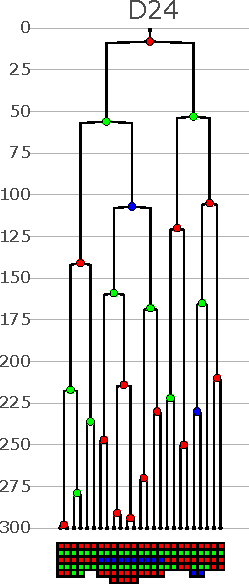
\includegraphics[width=0.18\textwidth]{images/cellLineage.pdf}
%	\end{center}
%\vspace{-20pt}
%\caption[]{\bf Lineage tree.}
%\vspace{-10pt}
%\label{fig:cellLineage}
%\end{wrapfigure}
%%
%\subsubsection{Periclinal Division Sequences}
%\label{sec:treeDivisionSequence}
%\noindent
%%
%\begin{figure}[htbp]
%	\begin{center}
%		\begin{overpic}[width=1.0\linewidth]{images/treeDivisionSequenceSample.pdf}
%		\end{overpic}
%\caption[]
%{
%{\bf Division sequence trees along the number of time points (left) and number of cells (right) for dataset \#120830.}
%}
%	\label{fig:treeDivisionSequenceSample}
%	\end{center}
%\end{figure}
%%

\clearpage
\section{Quantification and Visualisation of Lateral Root Primordium Deformation}
\noindent
The datasets served as a basis to perform an analysis of the lateral root deformation as a function of time. The analysis was inspired by the work of Graner~et~al.~\cite{graner_et_al_2008}. The idea is that the deformation can be computed using geometrical and topological properties of the underlying tissue. Since in our case we have a set of 3D cell nuclei for each time point (red nodes in Figure~\ref{fig:deformation}) that accurately mark the position of the cell (the nuclei do not move within a cell), we use their 3D positions to generate a triangulation (e.g. Delaunay triangulation) creating a surface that represents the tissue (see Figure~\ref{fig:deformation}). The deformation analysis can be performed object- or spatial-oriented. This means that either the deformation is evaluated and illustrated for each cell or the total area of interest is subdivided into regions of equal sizes to measure the deformation within each subregion. We consider the former case because we want to focus on individual cell changes. Besides, the initial number of cells in each dataset is quite small and therefore, the total area of interest is not covered by all cells which makes an object-oriented analysis per cell more reasonable.
%
\begin{figure}[htbp]
	\begin{center}
		\begin{overpic}[width=1.\linewidth]{images/deformation.pdf}
		\end{overpic}
\caption[]
{
{\bf Surface generation for deformation analysis.}
}
	\label{fig:deformation}
	\end{center}
\end{figure}
%

\subsection{Computation of Geometrical and Topological Contributions}
\noindent
The generated triangulation provides a neighbourhood information for each cell nucleus and we can further analyse the deformation of a cell over time. Let $c_1$ be one cell with position $p_{c_1} = ( x_1, y_1, z_1 )$. Another cell $c_2$ with position $p_{c_2} = ( x_2, y_2, z_2 )$ is a neighbour of $c_1$ if both share an edge or link $l = p_{c_2} - p_{c_1}$. Note that $l$ and $-l$ represent the same role of deformation but to be invariant under the change $l \rightarrow -l$, a \textit{link matrix} $m$ is used~\cite{graner_et_al_2008}:
\begin{equation}
m = l \otimes l =
\begin{pmatrix}
X^2 & XY & XZ\\
YX & Y^2 & YZ\\
ZX & ZY & Z^2
\end{pmatrix}
, \qquad
\left( X, Y, Z \right) = \left( x_2 - x_1, y_2 - y_1, z_2 - z_1 \right).
\end{equation}
This matrix incorporates the square link length and the angle by computing the tensor product of the link $l$. Further computations consider the average of all relevant links $N$ for a specific cell which is defined as the \textit{texture tensor}~\cite{aubouy_et_al_2003}:
\begin{equation}
M = \langle m \rangle = \langle l \otimes l \rangle = 
\begin{pmatrix}
\langle X^2 \rangle & \langle XY \rangle& \langle XZ \rangle\\
\langle YX \rangle & \langle Y^2 \rangle & \langle YZ \rangle\\
\langle ZX \rangle & \langle ZY \rangle & \langle Z^2 \rangle
\end{pmatrix}
= \mathlarger{\mathlarger{\nicefrac{\sum\limits_{N} l \otimes l}{N}}}.
\end{equation}
%
\begin{figure}[htbp]
	\begin{center}
		\begin{overpic}[width=1.\linewidth]{images/ellipseDeformation.pdf}
		\end{overpic}
\caption[]
{
{\bf Computation of deformation. Left:} 2D example of \textcolor{blue}{conserved}, \textcolor{red}{appearing} and \textcolor{green}{disappearing} links between two time points due two a cell division. {\bf Right:} Deformation is represented by the axes of an ellipse (ellipsoid) in 2D (3D).
}
	\label{fig:ellipseDeformation}
	\end{center}
\end{figure}
%

\noindent
The geometrical and topological terms are now computed by considering the variation of conserved, appearing and disappearing links between two time points $t$ and $t + \Delta t$ (see Figure~\ref{fig:ellipseDeformation}, left). More precisely, the geometrical variation, denoted as $B$ is computed by averaging the amount of conserved links $N_c$ between two time points~\cite{graner_et_al_2008}:
\begin{equation}
B = \frac{N_c}{N} \left\langle \frac{\Delta m}{\Delta t} \right\rangle = \frac{N_c}{N} \left\langle \frac{\Delta (l \otimes l) }{\Delta t} \right\rangle.
\end{equation}
This means that $M$ is evaluated at $t$ and $t + \Delta t$ and the difference is computed. For small $\Delta t$ values, $\frac{N_c}{N} \rightarrow 1$ because then almost all links $N$ are conserved and $B$ can then be written as:
\begin{equation}
B = \left\langle l \otimes \frac{dl}{dt} \right\rangle + \left\langle \frac{dl}{dt} \otimes l \right\rangle.
\end{equation}
The topological variation $T$ takes the averaging of the $N_a$ appeared and $N_d$ disappeared links into account depending on the corresponding averaged textures $\langle m_a \rangle$ and $\langle m_d \rangle$~\cite{graner_et_al_2008}:
\begin{equation}
T = \frac{1}{\Delta t} \left( \frac{\Delta N_a}{N} \langle m_a \rangle - \frac{\Delta N_d}{N} \langle m_d \rangle \right).
\end{equation}
The total deformation for each cell is then given by $B+T$. This sum is a matrix for which the eigenvalues $\lambda_i$ are computed. The magnitudes of these eigenvalues are proportional to the axes lengths of an ellipsoid that represents the spatial 3D deformation of a cell between $t$ and $t + \Delta t$ (see Figure~\ref{fig:ellipseDeformation}, right for a 2D case).
%
\begin{figure}[htbp]
	\begin{center}
		\begin{overpic}[width=1.\linewidth]{images/ellipseResults.pdf}
		\end{overpic}
\caption[]
{
{\bf Illustration of largest deformations by ellipses in dataset \#120830 (left) and \#121211 (right) in side view.}
}
	\label{fig:ellipseResults}
	\end{center}
\end{figure}
%
We compute the $B$ and $T$ terms for all 3D cell positions but we focus the visualisation on the 2D views using the side, front and radial views. Because of these 2D projections we illustrate the deformations by ellipses instead of ellipsoids in 3D for a more reasonable analysis. Figure~\ref{fig:ellipseResults} shows the resulting ellipses indicating the largest deformation (longest semi-axis) of two datasets right before the last time point.

\subsection{Averaging over Datasets}
\noindent
The above evaluation allows us to analyse the deformation of individual cells between two time points $t$ and $t + \Delta t$. Our intention is to analyse the averaged deformation of the lateral roots with respect to all five datasets. Note that we performed a spatial and a temporal registration of all datasets as described in Section~\ref{sec:registration}. The intersection range for the number of cells is $[18, 143]$. With this, the time point size $\Delta t$ is actually the variation of number of cells depending on the total number of considered steps $S$:
\begin{equation}
\Delta t = \frac{143 - 18}{S},
\end{equation}
and the current number of cell $s(i)$ for each step $i$ is:
\begin{equation}
s(i) = \left\lfloor s_i + 0.5 \right\rfloor, \qquad s_i = s_{i-1} + \Delta t, \qquad s_0 = 18.
\end{equation}
The usage of the floor function rounds $s(i)$ to the nearest integer value because $\Delta t$ might be a float value. However, it cannot be guaranteed that $s(i)$ appears in each dataset because of several cell divisions at one time point. We solve this issue by determining the nearest smallest possible cell number with respect to the current $s(i)$.
%
\begin{figure}[htbp]
	\begin{center}
		\begin{overpic}[width=1.\linewidth]{images/gridDeformation.pdf}
		\put(44.5,10.5){\small low}
		\put(55.1,10.5){\small high}
		\end{overpic}
\caption[]
{
{\bf Averaging over datasets and visualisation of deformation information. Left:} Example of how the deformation information of all datasets is averaged using a grid approach. {\bf Right:} Visualisation of averaged deformation information by colour-coded lines according to magnitude values given in Table~\ref{tab:deformationParameters} and ``bow ties'' over all datasets in side view. The black contour shows the convex hull using a B\'ezier curve.
}
	\label{fig:gridDeformation}
	\end{center}
\end{figure}
%

For each number of cell pair $s(i)$ and $s(i+1)$, $B+T$ is evaluated for each dataset resulting in the corresponding deformation information. To average it over all datasets we create a grid of tiles with constant but arbitrary dimension (see Figure~\ref{fig:gridDeformation}, left). For each tile in the grid we compute the average deformation of all ellipses whose centres are located in the corresponding tile. More precisely, the deformation in 3D given by all three axes of the ellipsoid is first averaged for each cell. Let $d_1, d_2, d_3$ be the three deformation vectors and $m_1, m_2, m_3$ the corresponding magnitudes. The average deformation $d_a$ and average magnitude $m_a$ per cell is then given by the mean:
\begin{equation}
d_a = \frac{1}{3} \sum_{i=1}^{3} d_i, \qquad m_a = \frac{1}{3} \sum_{i=1}^{3} m_i.
\end{equation}
Afterwards, the deformation vectors $d_a$ and the corresponding magnitudes $m_a$ of all $n$ cells located in the same tile are averaged:
\begin{equation}
D_a = \frac{1}{n} \sum_{n} d_a, \qquad M_a = \frac{1}{n} \sum_{n} m_a.
\end{equation}
As a result, each tile shows an averaged deformation represented by a line with normalized length. The averaged magnitudes are illustrated by a colour map and additional ``bow ties'' illustrate the variance of the deformation orientation (see Figure~\ref{fig:gridDeformation}, right).

We perform this averaging for all three views (front, side, radial). Figure 2B in the main text shows the deformation result for the first, mid and last time point ranges. For the front and radial view, we illustrate the deformation for all cells while for the side view we focus only on the cell changes located in the master cell file. Note that we determine in all cases the deformation information based on all 3D+t cell data. The magnitudes with unit $\boldsymbol{\nicefrac{\mu m}{min}}$ are in the range of $[0.0032, 0.1995]$ (front), $[0.0016, 0.1259]$ (side), and $[0.0016, 0.0501]$ (radial). We have chosen $S=20$ steps for which $\Delta t = 6.25$ with an average increase rate of $12.06$ cells per step. The deformation computation as well as the visualisation are realized in \textit{MATLAB}.

\clearpage
\section{Modelling of a Lateral Root Primordium Formation}
\noindent
We use a non-mechanical 2D vertex-based model for lateral root development. The evolving 2D tissue of the model is described by a graph, i.e.~an abstract structure in which a set of vertices is connected by a set of edges. In this context, an edge denotes a cell wall and a vertex corresponds to a junction that forms the point of contact between at least two cell walls~\cite{prusinkiewicz_lindenmayer_1990, prusinkiewicz_runions_2012}. As a consequence, the complete topology of all cells in the model (such as neighbourhood information) can be accessed via a graph rotation system~\cite{edmonds_1960}. We realize the implementation of the 2D model using \textit{OpenGL} (\href{https://www.opengl.org/}{https://www.opengl.org/}) and the \textit{VV} (Vertex-Vertex) programming language~\cite{smith_et_al_2004, smith_2006} which is embedded in a C{}\verb!++! programming environment.

%L-systems or also called Lindenmayer~Systems~\cite{lindenmayer_1968, prusinkiewicz_lindenmayer_1990}. The L-system is a language that consists of a set of strings based on predefined rules. More precisely, it consists of an axiom, the starting point of the system, and a set of production rules. The growth of a dynamic structure is realized by applying these rules to the axiom in which the resulting string is again in the language of the used system. Through this, the growth can be described by an infinite set of strings that 'steers' the growth behaviour. L-systems are commonly used to model plant growths as well as to generate fractals such as the Sierpinski triangle, for example.

We use a 2D model for two main reasons. First, we focus our analysis on the cells located in the master cell file. These cells contribute most to the growth of the primordium and feature the property that they are mostly located within a plane in 3D. Thus, their 3D locations can be projected onto a 2D plane in side view without (too much) loss of information. Second, such a model is much easier to describe than a 3D model which significantly reduces the complexity and therefore simplifies the analysis. Our intention is the creation of an idealised model based on simple rules that allows a comparison to the datasets.

\noindent
Our model requires the application of a underlying \textbf{model surface} that represents the developing lateral root. Furthermore, the positioning and the number of \textbf{founder cells} that contribute to the development have to be determined. Additionally, the \textbf{rules for cell division events} have to be defined, i.e.~the type and time point of a division event. The simulation starts with a predefined number and positioning of founder cells and develops over time based on the underlying surface structure. During the simulation, the model surface and the cells within grow and increase in area. According to the chosen division properties, a cell divides if it exceeds a specific area threshold or area ratio with respect to its initial size right after its birth. Through this, we generate a convenient model representing the growth of the lateral root.

In the next sections, we will describe the underlying model surface and the settings for the initial founder cells and divisions. Afterwards, we explain the different model scenarios addressed in the main text.

\subsection{Model Surface}
\noindent
The choice of the underlying surface for the model fundamentally affects the development of the tissue. This means that a change of vertex positions on the surface influences the walls and junctions of all cells in the model. In our case, we use \textit{B\'ezier surfaces} to create an idealised model that allows the investigation of a common growth behaviour of the lateral root~\cite[supplement]{smith_bayer_2004}.
%The first one is used to create a triangulation based on real nuclei positions in the dataset for each time point. Through this, we can generate a data-driven model that incorporates the deformation behaviour of the nuclei and are able to compare the result with the real-world datasets.
%\subsubsection{Triangle Mesh}
%\noindent
%For each real-world dataset, we create a set of 2D triangle meshes. This means that for each time point, we generate a triangulation based on the corresponding real nuclei positions located in the master cell file only because these are mainly responsible for the overall dome-like structure of the VLR. Through this, the triangulation captures the temporal displacement and growth behaviour of the nuclei which is then further used in the model to dictate the simulation and tissue growth (see Figure~\ref{fig:surfaceGeneration}). More precisely, the cells in the model consists of changing junctions that are affected by the triangle changes. If a junction $j$ of a cell is located within a specific triangle then $j$ is given uniquely by a convex combination $j = \lambda_1 r_1 + \lambda_2 r_2 + \lambda_3 r_3$ of the three triangle vertices $r_i$. The $\lambda_i$ $\left( \sum_{i=1}^{3} \lambda_i = 1, \lambda_i \geq 0 \; \forall i \right)$ are called the barycentric coordinates of $j$ with respect to the triangle. In the model itself, a lot of conversions between these barycentric and Cartesian coordinates occur to compute the changing cells.
%%
%\begin{figure}[htbp]
%	\begin{center}
%		\begin{overpic}[width=1.\linewidth]{images/surfaceGeneration.pdf}
%		\end{overpic}
%\caption[Generation of triangle mesh based on real nuclei displacements.]
%{
%{\bf Generation of triangle mesh based on real nuclei displacements.}
%}
%	\label{fig:surfaceGeneration}
%	\end{center}
%\end{figure}
%%
%
%The triangulation can be either realized by a Delaunay triangulation or an $\alpha$-shape. Since we are only using the nuclei to construct the triangulation we require some additional information to of the VLR contour. Therefore, for each dataset, we manually generate a set of contour points to approximate the boundary of the VLR for the first (bottom left image in Figure~\ref{fig:surfaceGeneration}) and the last (bottom right image in Figure~\ref{fig:surfaceGeneration}) time point. We choose a constant number of 16 points such that the contour points for the time points in between are interpolated linearly (see bottom mid image in Figure~\ref{fig:surfaceGeneration}).
%%
%\begin{figure}[htbp]
%	\begin{center}
%		\begin{overpic}[width=0.8\linewidth]{images/surfaceMapping.pdf}
%%			\putIndex{0}{0}{A.pdf}
%%			\putIndex{52}{0}{B.pdf}
%		\end{overpic}
%\caption[Mapping of triangles and nuclei between subsequent time points.]
%{
%{\bf Mapping of triangles and nuclei between subsequent time points.} Nuclei displacements only do not interfere the bijectivity requirement but cell divisions do result in more triangles.
%}
%	\label{fig:surfaceMapping}
%	\end{center}
%\end{figure}
%%
%
%For the set of generated meshes, a bijective mapping of the triangles between time point $t$ and $t+1$ is required for the computation of arbitrary cell positions in between in the model. This means that each nuclei position in time point $t+1$ is uniquely assigned to a previous position in time point $t$ (top left in Figure~\ref{fig:surfaceMapping}). More precisely, our approach requires that we use the same triangulation (but with different nuclei positions) for subsequent time points. However, cell divisions may result in more nuclei in the next time point and consequently in more triangles (top right in Figure~\ref{fig:surfaceMapping}) impairing the bijectivity. To overcome this issue, for each occurring cell division, the average position of the two daughter cells (grey nodes) is computed at the next time point and represents a single nuclei position (cyan node) that can be bijectively mapped to the previous dividing cell (green node). At time point $t+2$, the two triangles originally created at $t+1$ are considered and the next time point $t+3$ is checked again. In total, there are two triangle meshes for each pair of subsequent time points that guarantee a bijective mapping which are between time point $t$ and $t+1$, as well as $t+2$ and $t+3$, respectively.
%
%The exchange of the different triangle meshes between $t+1$ and $t+2$ is realized by another approach. Consider the simplified model with three cells in Figure~\ref{fig:triangleExchange} and the inner junction $j$ in the model. At time point $t$, the position of $j$ is computed by its barycentric coordinates within the blue-rimmed triangle. When in the next time point the triangle mesh should have changed then it will be checked in which triangle $j$ is located now. Based on the position in the newly found blue-rimmed triangle, the new barycentric coordinates are computed. In further steps, either only a bijective mapping between two equal triangulations is needed or the same approach is applied facing a new triangle mesh. Note that at the beginning of the model, the setting of cells as well as their positions have to be defined manually. Based on these positions, the triangles are identified in which the junctions are located and the barycentric coordinates are computed.
%%
%\begin{figure}[htbp]
%	\begin{center}
%		\begin{overpic}[width=0.8\linewidth]{images/triangleExchange.pdf}
%%			\putIndex{0}{0}{A.pdf}
%%			\putIndex{52}{0}{B.pdf}
%		\end{overpic}
%\caption[Transition between two different triangle meshes.]
%{
%{\bf Transition between two different triangle meshes.} For each junction position $j$, the triangle of the underlying surface has to be identified in which $j$ is located at time point $t+1$. The red nodes indicate the nuclei while the black ones denote the contour points.
%}
%	\label{fig:triangleExchange}
%	\end{center}
%\end{figure}
%%
A two-dimensional B\'ezier surface of degree $(n, m)$ with $(n+1) \cdot (m+1)$ control points $c_{i, j} \in \mathbb{R}^2$ is a parametric surface that maps the unit square into a smooth-continuous surface embedded in the same space as its control points. Each point $P(u, v) \in \mathbb{R}^2$ on such a B\'ezier surface $S_{cur}$ with parametric coordinates $u ,v \in [0,1]$ is computed by the following equation:
\begin{equation}
P(u, v) = \sum_{i=0}^{n} \sum_{j=0}^{m} B_{i}^{n} (u) \; B_{j}^{m} (v) \; c_{i,j}, \qquad B_{i}^{n} (u) = \binom{n}{i} u^i (1-u)^{n-i}.
\end{equation}
As a consequence, given only a pair of B\'ezier surfaces $S_{first}$ and $S_{last}$ to describe the first and the last time point of the model, the surface at each other time point in between is computed by a linear interpolation of the control points $a_{i,j} \in S_{first}$ and $b_{i,j} \in S_{last}$:
\begin{equation}
c_{i,j} = (1-t) \cdot a_{i,j} + t \cdot b_{i,j}, \qquad \forall i, j \in [0, n], [0, m],
\end{equation}
with the control points $c_{i,j}$ of the current B\'ezier surface $S_{cur}$ and $t \in [0,1]$ as the temporal interpolation factor. By this, only two B\'ezier surfaces need to be generated manually for the model while the B\'ezier surfaces in between are given by interpolation which ensures a smooth growth behaviour of the model. Another advantage of using this kind of surface is that the mapping of each pair of parametric coordinates $u_i, v_i$ to a 2D position on the surface is unique although of course the developing surface structure will change over time (see Figure~\ref{fig:modelSurface}).
%
\begin{figure}[htbp]
	\begin{center}
		\begin{overpic}[width=0.8\linewidth]{images/modelSurface.pdf}
		\end{overpic}
\caption[]
{
{\bf First and last B\'ezier surfaces of degree $(6, 6)$ for the idealised model.} The mapping of $(u_i, v_i)$ to the changing position on the surface is unique over time.
}
	\label{fig:modelSurface}
	\end{center}
\end{figure}
%

\subsection{Configuration of Founder Cells}
\label{sec:founderCells}
\noindent
For the model we have to set the number and spatial properties of founder cells of the lateral root.
%\subsubsection{Data-driven Models}
%\noindent
%The first setting is designed in such a way that a valid comparison between model and real world dataset is achieved. The underlying surface of the model is a triangle mesh based on real nuclei positions as explained above. Furthermore, the number of cells in the model is selected such that it approximately matches the same number of cells in the real-world datasets for both, the beginning and the end of the given datasets. In order to preserve the same number of cells at the end in the model, we steer the parameter for the division event as explained later.
We consider two different model configurations at the beginning. In the first one, the model starts with two founder cells of equal sizes and shapes (see Figure~\ref{fig:founderCellsSetting}, left) which develops depending on the selected division rules explained in Section~\ref{sec:divisionRules}. The second configuration is identical to the first one but we force the first division to be an asymmetric anticlinal one (see Figure~\ref{fig:founderCellsSetting}, right). More precisely, the inner daughter cells share the same size but with only one third of the parents cell sizes.
%\begin{inparaenum}[(\itshape i\upshape)]
%\item The model with two founder cells of equal sizes (see Figure~\ref{fig:founderCellsSetting}, top left) develops depending on the selected division rules explained below.
%\item The start configuration is identical to (\textit{i}) but we force the first division to be asymmetric (see  Figure~\ref{fig:founderCellsSetting}, top right). More precisely, the inner daughter cells share the same size but with only one third of the parents cell sizes.
%\item Identical to (\textit{ii}) but we force the second division to be a symmetric periclinal one (see Figure~\ref{fig:founderCellsSetting}, bottom left).
%\item Identical to (\textit{ii}) but we force the second division to be a symmetric anticlinal one (see Figure~\ref{fig:founderCellsSetting}, bottom right).
%\end{inparaenum}
%Note that for the first and second division rounds the VLR model already started to evolve and eventually changed its tissue structure. For the sake of clarity, Figure~\ref{fig:founderCellsSetting} only covers the division scenarios without any evolution of the tissue.
%
\begin{figure}[htbp]
	\begin{center}
		\begin{overpic}[width=0.8\linewidth]{images/founderCellsSetting.pdf}
		\end{overpic}
\caption[]
{
{\bf Two initial founder cell configurations for the model.}
}
	\label{fig:founderCellsSetting}
	\end{center}
\end{figure}
%

\subsection{Division Events}
\noindent
In the model, time point and axis orientation of each division have to be determined. We use non-deterministic division rules for each model, i.e.\ a random variation of orientation of the division axis. By repeated simulations (e.g.\ 100) of such a probabilistic model with the same setting we can analyse its division behaviour based on statistically solid results.

\subsubsection{Time Point of Division}
\noindent
At each time point of the model simulation, the area of each cell is computed and compared with its initial area. If the cell's area exceeds the initial area by a certain amount a division event will occur. This amount is determined by setting an \textit{area ratio} and an \textit{area threshold}. The ratio defines the maximal percentage increase of a cell before it should divide. For example, a ratio of $0.5$ denotes that the cell will divide if its initial size has increased by at least $50\%$. However, only using this ratio would result in cell areas that converge to zero in later steps because the percentage ratio above would result in smaller cells over time. For this reason, the area threshold is used as a barrier to guarantee a minimum area for each cell before it divides.

\subsubsection{Orientation of Division Axis}
\label{sec:divisionRules}
\noindent
After defining the time point of a division event we need to set the orientation of the division axis. In our model, we consider two division rules which we refer to as Besson-Dumais rule and random rule.
%\begin{Itemize}
%\item Besson-Dumais (BD),
%\item Alternating plane of division (D) + random variation,
%\item Perpendicular to principal direction of growth (PDG) + random variation,
%\item Random (R) and,
%\item Random with equal daughter cell sizes (RE).
%\end{Itemize}
%
\begin{figure}[htbp]
	\begin{center}
		\begin{overpic}[width=0.6\linewidth]{images/divisionRules.pdf}
		\end{overpic}
\caption[]
{
{\bf  Besson-Dumais division rule.}
}
	\label{fig:divisionRules}
	\end{center}
\end{figure}
%

The Besson-Dumais division rule~\cite{besson_and_dumais_2011} can be seen as a generalization of the shortest wall or Errera's rule~\cite{errera_1886} which will always result in the shortest division axis that can be generated to connect two opposing cell walls through the centre of mass (red dots in Figure~\ref{fig:divisionRules}). Using this rule, each axis orientation of a set of $N$ possible orientations is assigned a specific probability value based on the length $l_i$ of the line and the cell's area $A$:
\begin{equation}
p_i = \frac{e^{-\beta l_i / \rho}}{\sum_{j=1}^{N} e^{-\beta l_j / \rho}}.
\end{equation}
$\rho = \sqrt{A}$ is the mean cell diameter and $\beta = 20.6$ is a parameter that was empirically determined by Besson and Dumais~\cite{besson_and_dumais_2011} for which the proportion of cells dividing along the shortest wall is supported by this value. As a consequence, we have a probability distribution function for the set of division axes and the axis with the highest probability is identical with the shortest one. Figure~\ref{fig:divisionRules} illustrates three examples of division orientations and their corresponding colour-coded probabilities.

%The next scenario is in choosing a division axis that is perpendicular to the principal direction of the cell's growth \textbf{(PDG)}. More precisely, a set of changing centre of mass positions for each cell since its birth and right before it divides is gathered. For this set, the principal component is computed and the next division axis is then perpendicular to this principal direction. However, the whole division behaviour is deterministic and we therefore include a randomized variation of the division orientations by defining a random angle range $[-\alpha, \alpha]$. After determining the division axis, its orientation is varied by a randomly chosen angle value within this range (see Figure~\ref{fig:divisionRules}, PDG). The model result with $\alpha = 10$ is given in Figure~\ref{fig:suppmodel}G-I.

%The alternating plane of division rule \textbf{(D)} will result in a division axis that is always perpendicular to the previous division axis of the parent cell. The initial division orientation is given by the setting of the founder cells. Thus, equal to PDG, using this rule result in a deterministic division behaviour which is always the same for each repeated model simulation. Consequently, we add a randomized variation of the division orientation (see Figure~\ref{fig:divisionRules}, D). Note that the interphase duration between these two division events take some time in which the cell's size is increasing. However, in Figure~\ref{fig:divisionRules}, D, the cell has the same size and shape in the next division round for the sake of clarity. The model result with $\alpha = 10$ is given in Figure~\ref{fig:suppmodel}J-L.

In contrast, the random rule generates arbitrary division axis orientations through the centre of mass with respect to a cell-shape preserving property that is explained in Section~\ref{sec:cellShape}. All possible division orientations have the same probability.

%We also considered a division rule that is identical to R but which preserves almost equal areas of the daughter cells \textbf{(RE)}. Note that when using only straight lines as division walls a perfect splitting of a cell into two equal areas is not always satisfied. As a consequence, it cannot be guaranteed that the division axis is in a right angle to both connected cell walls. But for simplification in the model analysis we stick to a straight division axis and not to a curved one. If a division orientation is chosen randomly, the two resulting daughter cell areas $A_1, A_2$ are computed with respect to their parent cell's size $A$ and the percentage values $p_1, p_2$ are compared with each other:
%\begin{equation}
%p_1 = \nicefrac{A_1}{A}, \qquad p_2 = \nicefrac{A_2}{A}.
%\end{equation}
%If $| p_1 - p_2 | > \eta$ with $\eta$ a user-chosen threshold then a new division orientation is randomly chosen until this inequality is satisfied (with a maximum number of attempts $N$ to avoid infinity loops). A model result is given in Figure~\ref{fig:suppmodel}D-F with $\eta = 10$ and $N=50$.

\subsubsection{Classification of Division Type}
\label{sec:ClassificationOfDivisions}
\noindent
In our 2D model, we are able to classify a division type either as an anticlinal or a periclinal one. We realize this by investigating the orientation of the division axis with respect to a unit vector $(0,1,0)$ that corresponds to the y-axis. Figure~\ref{fig:divisionClassification} illustrates the idea and we classify the division type according to the following angle computation:
\begin{equation}
\alpha =
\begin{cases}
\measuredangle \left( \frac{p-q}{\lVert p-q \rVert}, (0,1,0) \right) & \text{if}\; p.y \geq q.y,\\
\measuredangle \left( \frac{q-p}{\lVert q-p \rVert}, (0,1,0) \right) & \text{else}.\\
\end{cases}
\end{equation}
If the angle $\alpha$ is smaller or equal than some angle threshold then the division is an anticlinal one, else it is a periclinal division. We use an angle threshold of $45$ degrees in all models.

%
\begin{figure}[htbp]
	\begin{center}
		\begin{overpic}[width=0.5\linewidth]{images/divisionClassification.pdf}
		\end{overpic}
\caption[]
{
{\bf Classification of division type in our models.}
}
	\label{fig:divisionClassification}
	\end{center}
\end{figure}
%

\subsection{Model Scenarios}
\label{sec:modelScenarios}
\noindent
Using the B\'ezier surfaces, the setting of founder cells as well as the division properties, we are able to create a model of the lateral root. We research how the division behaviour is influenced when cells are dividing based on a specific rule or randomly. Furthermore, we investigate the robustness of the model when changing certain properties. For all models, we choose an initial configuration with two founder cells that have equal areas and shapes (see Figure~\ref{fig:founderCellsSetting}, left). In total, we consider six different model scenarios:

\noindent
\textbf{Model 1: Geometric}\\
\noindent
In Model 1, the division axes are chosen based on the Besson-Dumais division rule described in Section~\ref{sec:divisionRules} (see Figure 1A-C in main text).

\noindent
\textbf{Model 2: Random}\\
\noindent
For Model 2, the orientation of the division axes are chosen randomly for all divisions (see Figure 5D-F in main text and Figure~\ref{fig:visumodel}).

\noindent
\textbf{Model 3: 1\textsuperscript{st} random then geometric}\\
\noindent
In Model 3, we randomise the orientation of the division axes in the first division round and use the Besson-Dumais division rule for all subsequent divisions (see Figure 5G-I in main text and Figure~\ref{fig:visumodel}). By this, we can analyse the robustness of the model development with respect to the first division round.

\noindent
\textbf{Model 4: Basal growth}\\
\noindent
Model 4 is designed to check whether the lateral root growth itself is responsible for the emergence of the observed sequence of periclinal divisions. For this purpose, we change the deformation behaviour of the B\'ezier surface from an equidistant distribution of control points to a distribution in which the control points are growing faster towards the dome tip (see Figure~\ref{fig:basalGrowth}). We force the first division round to be an asymmetric anticlinal one (see Figure~\ref{fig:founderCellsSetting}, right) and we use the Besson-Dumais rule for subsequent divisions. As a result, the model leads to more dominant cell divisions at the base of the primordium. This model impairs the high-order pattern of periclinal divisions (see Figure 5J-L in main text and Figure~\ref{fig:visumodel}) although the layer formation and division orientations are similar to the model results using an equidistant distribution of control points.

\noindent
\textbf{Model 5: 1\textsuperscript{st} asymmetric then geometric}\\
\noindent
In Model 5, we force the first division round to be an asymmetric anticlinal one yielding pairs of daughter cells with volume ratios of 2:1 (see Figure~\ref{fig:founderCellsSetting}, right). The Besson-Dumais division rule is used for all subsequent divisions (see Figure~\ref{fig:Modelsupp}).

\noindent
\textbf{Model 6: Random with equal areas}\\
\noindent
For Model 6, the orientation of the division axes are chosen randomly for all divisions but for each division axis the resulting areas of the two daughter cells are computed and compared with each other. If the areas differ in more than $10\%$ then a new division axis is chosen randomly and the areas are checked again. If no division axis results in almost equal areas after $50$ attempts, the last randomly generated one is chosen (see Figure~\ref{fig:Modelsupp}).

%
\begin{figure}[htbp]
	\begin{center}
		\begin{overpic}[width=1.\linewidth]{images/basalGrowth.pdf}
		\end{overpic}
\caption[]
{
{\bf Growth behaviour of the surface model. Left:} Equidistant distribution of control points in a B\'ezier surface. \textbf{Right:} Basal growth of the model which impairs the high-order pattern of periclinal divisions.
}
	\label{fig:basalGrowth}
	\end{center}
\end{figure}
%

\subsubsection{Model Simulation}
\noindent
For each model scenario, we perform $100$ simulations with $500$ model steps (time points) to test how stable the model and therefore the division results are based on the randomised variations of the division rules. Furthermore, we use a constant area threshold value of $1100$ while the area ratio is chosen in such a way that at the end approximately $64$ cells are generated. This value originates from the average number of cells in the master cell file for all five wild type datasets ($(64+49+81+46+82)/5 \approx 64$). Table~\ref{tab:modelParameters} lists all area ratios, average numbers of cells, anticlinal and periclinal divisions for each model scenario.

\subsection{Model Modifications}
We apply some modifications to the model that affect the resulting tissue and cells in order to better approximate a real-world behaviour.
%
\begin{figure}[htbp]
	\begin{center}
		\begin{overpic}[width=0.7\linewidth]{images/shapePreserving.pdf}
		\end{overpic}
\caption[]
{
{\bf Cell Shape Preservation.} For each division axis through the centre of mass rotated by an user-selected angle $\alpha$, a length check of the connected cell walls is applied. For this purpose, the two interconnecting nodes $u$ and $v$ as well as the adjacent junctions $u_1, u_2$ and $v_1, v_2$ are determined. From these positions the lengths $a, b, c, d$ and the cell wall lengths $a+b$ and $c+d$ are computed. It is then checked which of the four cases $a < (a+b)\cdot \delta$, $b < (a+b)\cdot \delta$, $c < (c+d)\cdot \delta$, or $d < (c+d)\cdot \delta$ is true. If only one statement is false then this division axis orientation is omitted. The user-selected value $\delta$ is in the range $[0,1]$ and denotes the percentage that a sub-line must have with respect to the total cell wall length.
}
	\label{fig:shapePreserving}
	\end{center}
\end{figure}
%

\subsubsection{Cell Shape Preservation}
\label{sec:cellShape}
\noindent
In the model, a total random configuration of cell division axes may result in implausible cell developments with unequal sizes and triangle-shaped contours that cannot be observed in any real-world scenario of plant growth. We want to analyse a random behaviour of cell divisions that somehow preserve equal sizes and shapes of cells after divisions. We therefore first find a set of division axis orientations that satisfy a specific constraint and assign each one the same probability value. The idea of this approach is explained in Figure~\ref{fig:shapePreserving}. We use a value of $\delta = 0.15$ for the random division rule while this approach is not applied to the Besson-Dumais rule because there we do not observe any implausible cell shapes.

\subsubsection{Computation of Centre of Mass}
\noindent
Note that for all division rules the division axis always passes through the centre of mass. However, in later model steps, more and more cells are created that share several junctions (see Figure~\ref{fig:levelOfDetail}, left).
%
\begin{figure}[htbp]
	\begin{center}
		\begin{overpic}[width=1.\linewidth]{images/levelOfDetail.pdf}
		\end{overpic}
\caption[]
{
{\bf Modified computation of centre of mass. Left:} The centre of mass of cells with several junctions may not yield a ``real'' centre of the cell. \textbf{Right:} A triangle fan is generated to compute a more adequate centre of the cell (green node) using the triangle centres of mass (blue nodes) and their areas.
}
	\label{fig:levelOfDetail}
	\end{center}
\end{figure}
%
Consequently, a cell consists of more junctions and the computed centre of mass will be located near the mass of junctions (cyan node in Figure~\ref{fig:levelOfDetail}, left). This may result in an implausible division axis that also does not preserve equal areas of daughter cells. In order to solve this issue, we generate a triangle fan with one central vertex given by the initial centre of mass (see Figure~\ref{fig:levelOfDetail}, right). We then compute the areas $A_i$ and centres of mass $c_i$ of all triangles $i \in [1,n]$ and use this information to get a more adequate centre of the cell with respect to the total area $A$ of the cell:
\begin{equation}
c = \sum_{i=1}^{n} \left( c_i \cdot \frac{A_i}{A} \right).
\end{equation}
%perform a \textit{level of detail} of cell walls using the \textit{edge criterion}~\cite{jenks_1989} in such a way that only these junctions are preserved that mainly capture the shape of the cell. For example, the cell in Figure~\ref{fig:levelOfDetail} has seven junctions. Performing a level of detail results in a simplified cell shape that only has four remaining junctions (see Figure~\ref{fig:levelOfDetail}, right) while preserving the overall shape of the cell. The centre of mass is then computed based on these remaining junctions. A detailed description of the algorithm can be found in \cite[p.\ 59--60]{FangerauDiss_2015}. Note that we apply this level of detail only for the computation of the centre of mass. We do not remove any junctions of cells in the model itself.

\subsubsection{Smoothness of Model Surface}
\noindent
One initial cell consists of four junctions defining a rectangular cell shape within the underlying tissue.
%
\begin{figure}[htbp]
	\begin{center}
		\begin{overpic}[width=1.\linewidth]{images/subdivision.pdf}
		\end{overpic}
\caption[]
{
{\bf Subdivision approach for tissue modelling. Top:} Using only six junctions (red nodes) for two cells result in an implausible tissue model based on the underlying B\'ezier surface. \textbf{Bottom:} Creating more inner junctions (cyan nodes) result in a much smoother tissue development.
}
	\label{fig:subdivision}
	\end{center}
\end{figure}
%
For example, consider the first B\'ezier surface with two cells at the first model step resulting in six junctions (two are shared by the cells) with their corresponding parametric coordinates (see Figure~\ref{fig:subdivision}, top left). In a later model step, the tissue will start to grow evolving into the dome-like structure (see Figure~\ref{fig:subdivision}, top right). However, only the junction with the parametric coordinate $(u=\nicefrac{1}{2}, v=1)$ will move upwards based on the underlying B\'ezier surface creating a triangle-shaped tissue. In order to better embed the underlying surface into the model, additional inner junctions (cyan nodes in Figure~\ref{fig:subdivision}, bottom left) are created that result in a much smoother surface of the model (see Figure~\ref{fig:subdivision}, bottom right). This smoothness is defined by a user-chosen subdivision level which is $4$ in all our models and yields $2^{4-1} - 1 = 7$ additional inner junctions.

%\subsection{Visual Analysis}
%\subsubsection{Visualisation of the Model}
%\noindent
%We realize the implementation of the 2D model using \textit{OpenGL} (\href{https://www.opengl.org/}{https://www.opengl.org/}) and the \textit{VV} (Vertex-Vertex) programming language~\cite{smith_et_al_2004, smith_2006} which is embedded in a C{}\verb!++! programming environment. For a visual analysis, we generate three different representations of the evolving cells in the VLR: Illustration of
%\begin{inparaenum}[(\itshape i\upshape)]
%\item all cell contours (see Figure~\ref{fig:modelVisualisation}, left),
%\item cells as spheres (see Figure~\ref{fig:modelVisualisation}, mid) and
%\item adjacent cell layers (see Figure~\ref{fig:modelVisualisation}, right).
%\end{inparaenum}
%%
%\begin{figure}[htbp]
%	\begin{center}
%		\begin{overpic}[width=1.\linewidth]{images/modelVisualisation.pdf}
%		\end{overpic}
%\caption[]
%{
%{\bf Representation of evolving cells in model.} The model result can be illustrated by cell contours, cell spheres or by cell layers.
%}
%	\label{fig:modelVisualisation}
%	\end{center}
%\end{figure}
%%
%The first representation shows the cell contour information within the evolving tissue. Each cell is coloured by its corresponding layer value. The positions of the rendered spheres are given by the centres of mass of each cell. The third representation displays the cell layers between adjacent cells that share the same layer value. Cells are adjacent if they share at least one common cell wall. The lines (cylinders) are drawn for at least two cells through the centres of mass of the corresponding cells. Figure~\ref{fig:visumodel} shows the visualisations for the last model step of the four model scenarios.

\subsection{Visual Division Analysis}
\label{sec:visualAnalysis}
\noindent
We run several simulations of one model using division rules with randomized variation, each resulting in one division sequence tree as shown in Figures~\ref{fig:treeDivisionSequencesCells} and~\ref{fig:treeDivisionSequences}. Multiple simulation runs of each model allow us to use statistically solid model results and to compare them with the datasets.
%
\begin{figure}[htbp]
	\begin{center}
		\begin{overpic}[width=0.4\linewidth]{images/averagedTreeDivisionSequence.pdf}
		\end{overpic}
\caption[]
{
{\bf Averaged division sequence tree.} In only $48 \%$ of the $100$ comparisons in total, the upper layers were generated before the lower ones resulting in a red rectangle. In the other two cases with fewer comparisons ($81$ and $92$), more than $74 \%$ of the upper layers were generated first and green rectangles are drawn.
}
	\label{fig:averagedTreeDivisionSequence}
	\end{center}
\end{figure}
%
For this purpose, we modify the visualisation of the division sequence trees. Let $l$ be the sequence length for a generated layer (e.g.\ $l=3$ for $012$). We replace the x-axis showing the time points by a fixed temporal layout of the tree in which the pair of upper concurrently generated layers (with identical number sequence except for the last number) always occur first (slight translation to the left) with respect to its lower layers with almost the same division sequence (except for the $(l-1)$-th number). For example, the pair of layers $0111/0112$ are combined because their sequences only differ in the last number. This pair is compared with the pair $0121/0122$ because they differ in the third ($l-1 = 4-1 = 3$) position of the sequence. For each such a comparison we render a rectangle that includes these two pairs of layers and its colour is set to red or green. The rectangle is green if in more than $50 \%$ of the model simulations the upper layer occurred first with respect to the lower one and else we colour it red. This allows an immediate visual feedback of the high-order pattern while detailed information about the percentage and number of possible comparisons are given in the mid of each rectangle (see Figure~\ref{fig:averagedTreeDivisionSequence}). A comparison between pair of layers is not possible if only one pair of layers is generated or none at all. We also use a simplified version of this tree when the number of simulations as well as the sequence labels can be ignored (see Figures 1B and 5B, E, H, K in the main text).
\clearpage
% renaming of references
\addto\captionsenglish{\renewcommand{\refname}{\section*{Supplemental References}}}
\renewcommand{\refname}{Supplemental References}
% list of sources included in the table of contents: 
%\addcontentsline{toc}{section}{%
% \numberline{}Supplemental References}
% using of own bibtex format
\bibliographystyle{bib/Science}
\bibliography{bib/lit.bib}

% end of document
\end{document}
